\documentclass[12pt,a4paper]{report} % класс выбран report, как наиболее подхоящий по структуре и оформлению

%\usepackage{lscape}		% Для включения альбомных страниц

\usepackage{amsmath,amsthm,amssymb, gensymb}  %подгрузка пакетов для корректного и наиболее полного. должен грузиться как можно раньше, т.\,к. внутри себя определяет шрифты и некоторые прочие настройки, которые несколько не соответствуют тому, что надо.

%\usepackage{mathtext} %позволяет использоваться текстовые кириллические индексы в формулах

\everymath{\displaystyle}   %отключаем мастабирование символов в многоэтажных дробях, индексах и пределах интегралов в соответствии с традицией русской типографской вёрстки

\DeclareMathSizes{12}{20}{14}{10}    %увеличенные размеры символов в формулах
\usepackage{hyperref}
\usepackage{afterpage}
\usepackage[warn]{mathtext}
\usepackage[T1,T2A]{fontenc}  %подгрузка расширенной поддержки кириллических шрифтов

\usepackage[utf8]{inputenc}    %прямым текстом указываем, в какой кодировке работаем (UTF8), применение других кодировок (cp1251 или koi8r) вполне допустимо, но не рекомендуемо (cp866 можно, но зачем?)

\usepackage[russian]{babel}    %указываем, что пользоваться будем русским языком, подгружающмя словари переносов, выставляются в соответствии с принятыми нормами отступы, интервалы между словами и пр.

\usepackage[left=30mm, right=15mm, top=20mm, bottom=20mm]{geometry}   %поля по ГОСТ Р 7.0.11-2011, пакет geometry воспринимает размеры в mm, cm, in и пр.

\usepackage{indentfirst}   %заставляет ТеХ делать отступ в первом абзаце главы/параграфа/раздела

\usepackage{setspace}   %пакет позволяет выставлять полуторные интервалы в тексте, но не вмешивается в подписи, таблицы и сноски

\usepackage{icomma}
\usepackage{multirow,makecell,array}	% Улучшенное форматирование таблиц

\usepackage{cite} % Красивые ссылки на литературу (конкретно, автоматическая сортировка и дефисы

\hyphenpenalty=10000%отключаем перенос 
\usepackage{graphicx} % Подключаем пакет работы с графикой
%\usepackage[dvips]{graphicx}
\usepackage{float}
\usepackage{tocloft}  %управление стилем оглавления

%увеличение шрифта с 12 pt по умолчанию, на 14 pt
\renewcommand{\tiny}{\fontsize{7}{8.4pt}\selectfont}
\renewcommand{\scriptsize}{\fontsize{9}{11pt}\selectfont}
\renewcommand{\footnotesize}{\fontsize{11}{13.6pt}\selectfont}
\renewcommand{\small}{\fontsize{12}{14.5pt}\selectfont}
\renewcommand{\normalsize}{\fontsize{14}{18pt}\selectfont}
\renewcommand{\large}{\fontsize{17}{20pt}\selectfont}
\renewcommand{\Large}{\fontsize{20}{25pt}\selectfont}

\makeatletter
\bibliographystyle{utf8gost705u}	% Оформляем библиографию в соответствии с ГОСТ 7.0.5
\renewcommand{\@biblabel}[1]{#1.}	% Заменяем библиографию с квадратных скобок на точку:
\makeatother

%реализация висячей пунктуации, соответствующей традиции русской типографской вёрстки
%\usepackage{microtype}
%\SetProtrusion
%{
%encoding = T2A,
%family = faq
%}
%{
%« = {1000,   },
%» = {  , 1000},
%„ = {1000,   },
%“ = {  , 1000},
%( = {1000,   },
%) = {  , 1000},
%! = {  , 1000},
%? = {  , 1000},
%: = {  , 1000},
%; = {  , 1000},
%. = {  , 1000},
%- = {  , 500},
%{,}= {  , 1000}
%}
%\DeclareMicrotypeSet{t2atext}{encoding=T2A}
%\UseMicrotypeSet{t2atext}

\renewcommand{\thechapter}{\arabic{chapter}.} 
\renewcommand{\thesection}{\arabic{chapter}.\arabic{section}.}
\renewcommand{\thesubsection}{\arabic{chapter}.\arabic{section}.\arabic{subsection}.}
\renewcommand{\thefigure}{\thechapter\arabic{figure}}
\renewcommand{\thetable}{\thechapter\arabic{table}}
\usepackage{hyperref}    %позволяет сделать в полученной PDFке рабочими ссылки как в оглавлении, так и в списке литературы и вообще в тексте

\setcounter{secnumdepth}{5}   %по правилам нумеруются все заголовки вплоть до пунктов, так что выставляется максимальная доступная по умолчанию глубина нумерации

\hyphenpenalty=10000%отключаем перенос 
\usepackage{titlesec}
\usepackage[usenames]{color}
\usepackage{colortbl}
%\usepackage{tempora}
\usepackage{pscyr}
\usepackage{newtxmath}
\renewcommand{\rmdefault}{ftm}  %а это установка нужного %нам шрифта
%\renewcommand{\rmdefault}{Times New Roman}

\begin{document}

\setlength{\parindent}{1.25cm} %настройка отступов
\sloppy   %убираем висячие строки  и подобное безобразие
\clubpenalty=10000		% Запрещаем разрыв страницы после первой строки абзаца
\widowpenalty=10000		% Запрещаем разрыв страницы перед последней строкой абзаца

\onehalfspacing   %полуторный интервал
\renewcommand{\cftchapdotsep}{\cftdotsep} %точки в оглалении между названиями глав и номерами страниц (по умолчанию их нет)

\renewcommand\bibname{СПИСОК ИСПОЛЬЗОВАННЫХ ИСТОЧНИКОВ}

\thispagestyle{empty}
\begin{center}
ФЕДЕРАЛЬНОЕ ГОСУДАРСТВЕННОЕ БЮДЖЕТНОЕ ОБРАЗОВАТЕЛЬНОЕ
УЧРЕЖДЕНИЕ ВЫСШЕГО ОБРАЗОВАНИЯ \\
<<МОСКОВСКИЙ ГОСУДАРСТВЕННЫЙ УНИВЕРСИТЕТ\\
имени М.В.ЛОМОНОСОВА>>

\vspace{.5cm}
ФИЗИЧЕСКИЙ ФАКУЛЬТЕТ\\
\vspace{.5cm}
КАФЕДРА ФИЗИКИ КОСМОСА\\
\vfill
БАКАЛАВРСКАЯ РАБОТА\\
\vspace{.5cm}
\Large
\textbf{<<Черенковский детектор электронов с энергиями 3--13 МэВ>>}
\large

\end{center}

\vfill

\begin{flushright}
Выполнил студент \\
414 группы\\
Разумов Александр Юрьевич\\

\underline{\hspace{3cm}}\\ %пример места для подписи

\vspace{1cm}

Научный руководитель:\\
к.т.н. Рубинштейн Илья Александрович\\
\underline{\hspace{3cm}}\\

\end{flushright}

\vfill
\begin{flushleft}
Допущена к защите \\
Зав. кафедрой \underline{\hspace{3cm}} \\
\end{flushleft}
\begin{center}
\vfill

\small МОСКВА \\ \number\year\normalsize
\end{center}

\newpage

\tableofcontents   %вставка оглавления

\phantomsection
%\titleformat{\chapter}
%{\filright}
%{\thechapter}
%{1em}{}

%\titleformat{\section}
%{\filright}
%{\thesection}
%{1em}{}

%\titleformat{\subsection}
%{\filright}
%{\thesubsection}
%{1em}{}


\chapter*{ВВЕДЕНИЕ}
 
\addcontentsline{toc}{chapter}{ВВЕДЕНИЕ} 

Настоящая работа посвящена моделированию и созданию черенковского детектора для регистрации ультрарелятивистских электронов.
В течение почти двух лет работа велась в трёх направлениях, объединённых одной тематикой и общей концепцией:
\begin{itemize}
	\item Литературный обзор. Под этим направлением следует понимать первые две главы настоящей работы, содержащих описание эффекта Вавилова-Черенкова, а также подробный список почти всех черенковских детекторов, использовавшихся в наблюдениях на искусственных спутниках Земли и других космических аппаратах. Рассмотрены различные варианты применения детекторов, приведены значимые  результаты.
	\item Экспериментальная часть. Эта часть посвящена созданию рабочего черенковского детектора электронов. Разработка прибора и его монтаж велись вместе с И.\,А. Рубинштейном. Представлены характеристики прибора и результаты первых экспериментальных тестов. Последующая экспериментальная работа была прекращена из-за осложнения эпидемиологической обстановки.
	\item Модельная часть. Это направление посвящено созданию модели прибора с заданными характеристиками с помощью комплекса программ GEANT4 на основе примера \textit{OpNovice}. Представлены результаты численного моделирования методами Монте-Карло различных процессов, происходящих при пролёте релятивистских электронов через прибор, даны оценки его эффективности. Была поставлена задача оценки спектрометрических свойств черенковского детектора с конструктивными дополнениями. 
\end{itemize}

\chapter{Излучение Вавилова-Черенкова}
\section{История открытия эффекта}

П.\,А. Черенков, будучи аспирантом С.\,И. Вавилова, обнаружил неизвестное свечение голубоватого света в прозрачных жидкостях под воздействием $\gamma$-излучения солей урана. Это произошло в 1934~г~\cite{Cerenkov}. Согласно предположению Вавилова, появление свечения имеет мало общего с хорошо изученной тогда люминисценцией; по его мнению, излучение вызвано торможением электронов, выбиваемых $\gamma$-лучами. Позже, в 1937~г., в работе И.\,Е. Тамма и И.\,М. Франка~\cite{Tamm} была объяснена природа явления,  впоследствии названного излучением Вавилова-Черенкова. Согласно их теории, свет испускается средой, через которую проходит заряженная частица со скоростью, превышающей скорость света $v=c/n$ в данной среде (где $c$ "--- скорость света в вакууме, а $n$ "--- коэффициент преломления). 

Как было сказано, природа эффекта имеет мало общего с люминисценцией. К тому времени основные закономерности люминисценции были установлены и сводились к следующему:
\begin{itemize}
    \item Спектральный состав люминисценции и её интенсивность зависят от типа вещества, температуры и его чистоты.
    \item Свет распространяется изотропно, т.\,е. не имеет выделенного направления.
    \item Малое изменение чистоты вещества, то есть концентрации примесей, способно уменьшить интенсивность свечения, так как уменьшается время жизни атома в возбужденном состоянии и увеличивается вероятность передачи этой энергии молекуле примеси.
    \item Поскольку люминисценция вызвана испусканием фотонов атомами при переходе из возбуждённого состояния на более низкий энергетический уровень, спектр излучения должен быть линейчатым.
\end{itemize}

Указанное излучение не обладало данными признаками. Как сообщается в статье Черенкова, излучение совершенно не зависело от температуры и чистоты вещества. Попытки <<тушить>> излучение растворением в веществе различных соединений не дали положительного результата. Стало ясно, что открытый эффект не относится к люминисценции. Дальнейшие эксперименты показали, что:
\begin{itemize}
    \item спектр излучения и интенсивность не зависят от чистоты вещества и температуры;
    \item излучение связано с движением электронов в среде;
    \item свет поляризован и направлен под небольшим углом к направлению пучка электронов;
    \item эффект имеет пороговый характер, так как не вызывается, например, электронами, рождёнными в веществе под действием рентгеновских лучей;
    \item спектр излучения непрерывен в излучаемом диапазоне длин волн.
\end{itemize}

В работе Тамма и Франка приведена полная математическая теория с постановкой задачи математической физики, итогом которой явилось обоснование существования этого эффекта. Проведём, не вдаваясь в математические выкладки, качественное объяснение некоторых свойств излучения. 

\begin{figure}[th]
	\noindent\centering{
		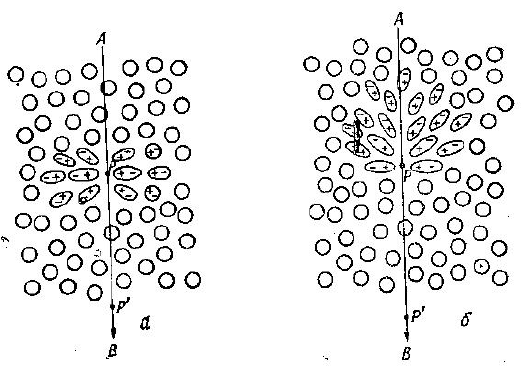
\includegraphics[width=120mm]{pictures/Polarisation.PNG}
	}
	\caption{Поляризация, возникающая в диэлектрике после прохождения заряженной частицы}
	\label{pic:Polarisation}
\end{figure}

Допустим, что электрон движется относительно медленно ($\beta n~<~1$) в прозрачной среде. В нормальном состоянии нейтральные атомы среды не возмущены и имеют приблизительно сферическую форму. В области, близкой к пролетающему электрону, его электрическое поле будет возмущать атомы, вследствие чего произойдёт частичная поляризация среды (см. рис. \ref{pic:Polarisation}). Если электрон покинет эту точку, спустя некоторое время среда вернётся в нормальное состояние. Пока атомы возмущены, они ведут себя подобно элементарным диполям, и во время пролёта электрона через среду каждый атом, расположенный рядом с его траекторией, получит кратковременный импульс. Так как поляризация среды относительно траектории пролёта будет симметрична (пренебрежём рассеянием электрона и неизбежным отклонением его от заданного курса), на больших расстояниях не будет результирующего поля.

Если электрон движется быстро (его скорость превышает фазовую скорость света в среде, $\beta n~ >~ 1$), то картина меняется. В этом случае не будет полностью симметричной поляризации, так как не будет осевой симметрии, только азимутальная. За столь краткое время пролёта электрона атомы-диполи не успевают развернуться назад.
Электромагнитные волны, излучаемые в разных точках траектории, оказываются когерентны, из-за чего в удалённой точке наблюдения возникает результирующее поле диполя, существующее даже на больших расстояниях. 
\section{Принцип работы черенковского детектора}

Весьма продолжительное время после открытия и объяснения этого эффекта не возникало идей его применения в экспериментальной физике. Среда испускает порядка нескольких сотен фотонов на каждый сантиметр пути заряженной частицы, и человеческому глазу  сложно увидеть какое бы то ни было излучение. Ситуация изменилась с появлением высокочувствительных фотоприборов "--- фотоэлектронных умножителей (ФЭУ). Первые возможные конструкции детекторов заряженных частиц на основе эффекта Вавилова-Черенкова были предложены в 1947 г.. В наше время эти детекторы используются в физике высоких энергий и для регистрации космических лучей.

Сформулируем основные черты черенковского излучения, которые обуславливают специфику детекторов, основанных на использовании этого эффекта:
\begin{itemize}
	\item Излучение имеет порог по энергии частицы, и порог зависит от оптических свойств вещества, в котором возникает свечение. Минимальная относительная скорость $\beta = v/c$, которой должна обладать частица, определяется отношением $\beta_{min} = 1/n$. Это позволяет различать частицы по их относительной скорости.
	\item Для большинства прозрачных сред в любом агрегатном состоянии излучение имеет сплошной спектр с максимумом в голубой части оптического диапазона.
	\item Излучение среды направлено под углом $\theta_c$ к вектору скорости заряженной частицы, где $\theta_c$ "--- половина угла раствора конуса черенковского излучения.
	 Косинус этого угла обратно пропорционален скорости частицы: 
\begin{equation} \label{costheta}
 \cos \theta_c = \frac{1}{\beta n}
\end{equation}
	\item Для мощности черенковского излучения справедлива формула Франка-Тамма:
\begin{equation} \label{FrankTammEquation}
 W = \frac{z^2 e^2 l}{c^2} \int_{\beta n(\omega)>1}
 \omega \left[ 1 - \frac{1}{\beta^2 n^2 (\omega)} d\omega \right]
\end{equation}
	\item Количество фотонов, излучаемых средой, пропорционально квадрату заряда пролетающей частицы $z^2$, что позволяет различать частицы по их заряду. Если считать постоянным показатель оптического преломления $n$, то в диапазоне волн с длинами от $\lambda_1$  до $\lambda_2$ на сантиметр пути частицы излучается количество фотонов $N$, рассчитываемое по следующей формуле (Джелли, \cite{Jelley}):
\begin{align}
& N = 2\pi\alpha z^2 \left( \frac{1}{\lambda_2} - \frac{1}{\lambda_1} \right)\overline{\sin^2 \theta_c},\label{N} \\
& N \approx 655 z^2 \cdot \overline{\sin^2 \theta_c}, \tag{\ref{N}$'$}
\end{align}
где $\alpha$ "--- постоянная тонкой структуры, а формула \ref{N}$'$ есть упрощённая формула для расчёта в диапазоне длин волн от 350 нм до 700 нм.
	\item Энергетические потери частицы на поляризацию среды и, следовательно, на черенковское излучение малы. 
\end{itemize}

Черенковский детектор включает в себя прозрачное вещество (радиатор), которое излучает свет при пролёте через него частицы, и фотоприёмник с высокой квантовой чувствительностью, способный зарегистрировать единичные фотоны. 

\section{Методика измерения}

Релятивистская заряженная частица, например, протон или электрон, влетает в прозрачное рабочее вещество детектора, или радиатор, и, если она обладает энергией, превышающей пороговую, в среде начинается излучение Вавилова-Черенкова.
Из-за существования выделенного направления света от частицы, регистрироваться будут только частицы, летящие в сторону фотокатода.
У некоторых детекторов алюминируется поверхность радиатора и чернится его верхний торец, чтобы снизить вероятность регистраций частиц, направленных от фотокатода.
Таким образом, доля излучённого света попадает на фотоприёмник, которым чаще всего является ФЭУ. 
К ФЭУ приложена ускоряющая разность потенциалов порядка 1 кВ. 
Количество черенковских фотонов пропорционально длине трека частицы в радиаторе. 
Падающий свет вызывает фотоэффект на катоде, и электроны, ускоряясь, попадают на диноды фотоприёмника, вызывая каскадное рождение фотоэлектронов. 
С последнего динода электроны попадают на анод, формируя отрицательный заряд. 
Заряд преобразуется в сигнал, сигнал инвертируется и усиливается, что в дальнейшем даёт возможность его анализа. Амплитуда сигнала пропорциональна заряду с анода, который, в свою очередь, зависит от количества фотонов, попавших на ФЭУ, т.\,е. от длины трека и скорости частицы.
\begin{figure}[th]
	\noindent\centering{
		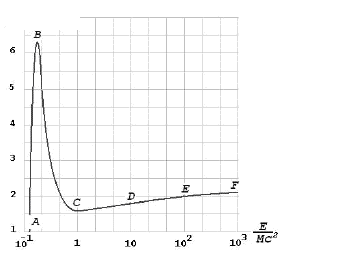
\includegraphics[width=120mm]{pictures/BetheBlokh.png}
	}
	\caption{Зависимость средних удельных ионизационных потерь тяжелой заряженной частицы на массовую единицу длины}
	\label{pic:BetheBlokh}
\end{figure}
Подобные детекторы имеют ряд преимуществ по сравнению с ионизационными детекторами, так как методы, основанные на ионизации среды, имеют очень ограниченный диапазон применимости. Если детектор является калориметром, и частица и все продукты её взаимодействия остаются в детекторе, то в этом случае вся энергия уходит на ионизацию среды. Зависимость ионизационных потерь от энергии имеет сложный вид, описываемый формулой Бёте-Блоха (\ref{BetheBloh}), и использовать эту зависимость для определения энергии частицы можно только на участке C--D (см. рис. \ref{pic:BetheBlokh}), где ионизационные потери частицы пропорциональны её энергии.

\begin{equation}\label{BetheBloh}
\left| \frac{dE}{dx}\right| = \frac{4\pi e^4}{m_e}\frac{z^2}{V^2}Zn_{ат}
\left[
	\ln \frac{2m_eV^2}{I(1-\beta^2)-\beta^2-\delta-u} 
\right] эрг\cdot см
\end{equation}

Здесь $z$ -- заряд частицы, $V$ "--- скорость частицы, $\beta = V / c$, плотность атомов $n_{ат}=\rho N_A/A~см^{-3}$, $N_A$ "--- число Авогадро, $\rho$ "--- плотность среды в $г/см^3$, $m_e$ -- масса электрона, а $I$ "--- средний потенциал ионизации для всех электронов среды. 

Дополнительная неопределённость при идентификации частицы по её ионизационным потерям возникает из-за их зависимости от квадрата заряда частицы $z^2$. Таким образом, несколько вторичных низкоэнергичных частиц могут имитировать пролёт релятивистской частицы с большим $z$. У детектора на основе эффекта Вавилова-Черенкова, в отличие от ионизационных детекторов, существует порог излучения, что позволяет частично разрешить эту проблему. 

В литературе (см.\cite{Ginzburg}) счётчики подразделяют на интегральные и дифференциальные. Интегральный счётчик "--- счётчик с одним порогом, регистрирующий все частицы с $\beta$ выше порогового. Дифференциальный счётчик обладает многими порогами и служит для получения дифференциального спектра, т.\,е. распределения ядер потока разного заряда по энергиям.

Для того, чтобы различать по заряду частицы, необходимо регистрировать амплитуду импульса с ФЭУ, вызванного вспышкой света от прохождения частицы через радиатор. 
Для дифференциального счётчика очень важно, чтобы их пути в веществе радиатора мало отличались друг от друга, так как число фотонов пропорционально пройденному частицей пути. 
Данное ограничение требует отбора частиц в очень малом телесном угле пролёта, так как если частица влетает в детектор даже под небольшим углом, серьёзно меняется количество фотонов, попадающих в ФЭУ, а следовательно, изменяется импульс на выходе. 
По этой причине требуется, чтобы пути частиц в детекторе мало отличались друг от друга.
Ограничение телесного угла достижимо, например, при настройке схемы совпадений с другими счётчиками, входящими в состав телескопа и задающими направление пролёта частицы.
Из всех импульсов с выхода фотоумножителя можно регистрировать только те, что соответствуют предшествующим импульсам с направляющих детекторов телескопа (например, с газоразрядных камер или сцинтилляционных счётчиков).
Вдобавок к этому, дифференциальный черенковский счётчик должен быть калориметром, т.\,е. для определения энергии, пропорциональной пути частицы, необходима остановка частицы в радиаторе в результате иониационных потерь.

У детекторов заряженных частиц существует также иная проблема, которая решается, если использовать их в связке с черенковским счётчиком.
Чем больше энергия первичной частицы, тем больше вторичных частиц образуется в веществе детектора.
Вторичные частицы рассеиваются и движутся во всех направлениях, в том числе и в направлении, противоположном движению первичной частицы. 
Этот эффект называется \textit{обратным током детектора}.
Возникают искажения получаемого спектра вследствие того, что вторичные частицы, движущиеся обратно, вызывают в основном детекторе (например, сцинтилляционном счётчике) ложные импульсы.
Так, например, несколько вторичных частиц могут по своему импульсу имитировать высокоэнергичный протон.
Решение этой проблемы требует фильтрации регистрируемых частиц по направлению, с чем прекрасно справляется черенковский детектор, который в телескопах выполняет функцию \textit{детектора направления}.
\chapter{Черенковские детекторы в космических детекторах}
В этой главе дан краткий литературный обзор почти всех черенковских детекторов, использовавшихся или используемых ныне в космических наблюдениях. Здесь не рассматриваются баллонные эксперименты по регистрации ядер космических лучей, несмотря на их большой вклад в науки о космических лучах.
\section{Советские черенковские детекторы в космосе}

\subsection{Спутник-3 и другие ИСЗ начала космической эры}

При помощи приборов, которые были установлены на советских космических спутниках и ракетах исследовался состав космических лучей вне земной атмосферы, а позже "--- вне магнитосферы. Первым научным прибором в космосе стал газоразрядный счётчик Гейгера-Мюллера на ИСЗ-2, на последующих спутниках устанавливалось больше научной аппаратуры. 

На третьем ИСЗ среди всей аппаратуры также были установлены счётчики интегрального типа (Гинзбург, Курносова и др.~\cite{Ginzburg}).
Для установки порогов использовались импульсы, создаваемые в детекторе мюонами и электронами космических лучей. 
Черенковский счётчик помещался в телескоп между серией газоразрядных счётчиков и включался в схему совпадений для того, чтобы сузить рассматриваемый телесный угол и избежать различия пробегов частиц, летящих под разными углами. Эти счётчики служили для регистрации ядер тяжёлых элементов в космических лучах. 


Согласно той же статье (см.~\cite{Ginzburg}), на ИСЗ-5 и ИСЗ-6, также неофициально называемых вторым и третьим кораблями-спутниками соответственно, были установлены два черенковских счётчика дифференциального типа и один интегральный. Интегральный счётчик второго корабля-спутника измерял относительную интенсивность ядер с $Z\geq5$ и $Z\geq15$, а дифференциальные счётчики регистрировали ядра от гелия до кислорода. 
На третьем корабле-спутнике была та же аппаратура, однако пороги интегрального счётчика были установлены так, что регистрировались ядра с $Z\geq5$ и $Z\geq12-14$.
По данным, полученным с интегральных счётчиков на ИСЗ-6, было установлено, что зависимости интенсивности лёгких ядер от геомагнитной широты почти совпадают друг с другом, что говорит о том, что энергетические спектры лёгких ядер подобны друг другу в той области энергий, где частицы подвержены геомагнитным эффектам. 
\begin{figure}[th]
	\noindent\centering{
		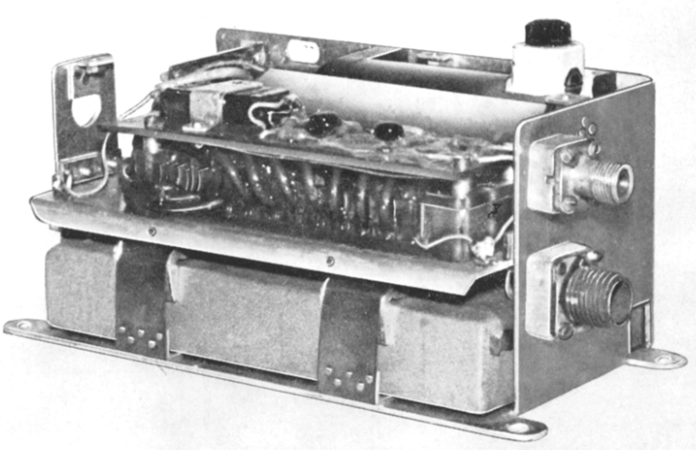
\includegraphics[width=70mm]{pictures/IntegralLunik2.PNG}
	}
	\caption{Внешний вид интегрального черенковского детектора, установленного на борту АМС <<Луна-2>>}
	\label{picLunik}
\end{figure}
К аппаратуре для изучения потоков ядер ещё можно отнести интегральные черенковские счётчики (см. рис. \ref{picLunik}) на борту АМС <<Луна-2>> и <<Луна-3>> (в литературе называются соответственно второй и третьей космическими ракетами). Во время полёта второй космической ракеты на этих счётчиках были зафиксированы кратковременные возрастания потоков ядер, связанные с хромосферными вспышками. 
На третьей космической ракете осуществлялось измерение потока ядер с большим зарядом ($Z\geq28$). 
Измерения в стратосфере показали, что потоки других тяжёлых ядер ничтожно малы в сравнении с потоками ядер из группы железа (Fe, Co, Ni).
\subsection{Спутники серии <<Протон>>}

Четыре советских искусственных спутника серии <<Протон>> были запущены в период 1965 "--- 1968 гг.
Первые эксперименты по непосредственному изучению частиц первичного космического излучения высоких энергий были осуществлены на научных станциях <<Протон-1>>, <<Протон-2>>, <<Протон-3>>. На этих станциях была установлена научная аппаратура для измерения общего энергетического спектра космического излучения до $10^{14}~эВ$ и энергетического спектра протонов до $10^{13}~эВ$.
\begin{figure}[th]
	\noindent\centering{
		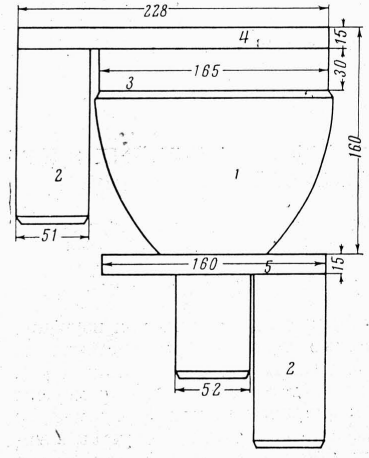
\includegraphics[width=70mm]{pictures/SEZ1.PNG}
	}
	\caption{Схематическое изображение спектрометра СЭЗ-1}
	\label{figSEZ1}
\end{figure}
На первых двух спутниках <<Протон-1>> и <<Протон-2>> были установлены черенковские спектрометры зарядов ядер СЭЗ-1 (рис. \ref{figSEZ1}), \cite{SEZ1}, состоявшие из черенковского детектора, расположенного между двумя сцинтилляционными счётчиками. Всё устройство работало как телескоп, включённый в схему совпадений. 
В качестве радиатора в черенковском счётчике использовался плексигласовый диск диаметром 165 мм и высотой 30 мм, а фотоумножителем является ФЭУ-49. 
Сцинтилляционные счётчики, в свою очередь, были составлены из ФЭУ-13 и пластических сцинтилляторов толщиной 15 мм. 
Противоположная от фотокатода сторона диска была зачернена для понижения вероятности регистрации частиц идущих в противоположную от ФЭУ сторону, а боковые стенки были покрыты белой эмалью во избежание выхода света. 
В схеме совпадений отбирались импульсы черенковского детектора, совпадающие по времени с импульсами от сцинтилляционных счётчиков. 
Градуировка прибора осуществлялась мюонами космических лучей на уровне моря. 
В течение трёх месяцев работы прибора на орбите было получено много информации о ядерном составе лучей для зарядов $Z=40\div50$. Были измерены спектры разных элементов в космических лучах в широком диапазоне. 

В состав аппаратуры ИСЗ <<Протон-1>> и <<Протон-2>> также входил спектрометр электронов – прибор СЭЗ-12, предназначенный для регистрации электронов с энергиями $E_e \geq 300$ МэВ и измерения их спектров \cite{SEZ12}. Спектрометр представлял собой телескоп из двух сцинтилляционных счётчиков и газового черенковского счётчика, где в качестве радиатора был фреон-13 под давлением 11 атм. Черенковский счётчик выполняет две функции. Во-первых, он регистрирует только те частицы, энергия которых не ниже пороговой. Во-вторых, он регистрирует частицы, идущие в телескопе в направлении от первого детектора ко второму, и не регистрирует частицы, идущие в обратном направлении. С помощью СЭЗ-12 получена широтная зависимость интенсивности электронов за пределами атмосферы. 

Как указывалось ранее, для борьбы с эффектом обратного тока необходимо фильтровать частицы по направлению прихода, т.\,е. использовать детектор направления. В качестве него черенковский детектор вошёл в состав телескопа СЭЗ-14  на спутнике <<Протон-3>>. Это был ионизационный калориметр, дополненный несколькими детекторами направления, каждый из которых состоял из четырёх черенковских счётчиков. Радиаторами были плексигласовые диски диаметром 16 см и толщиной 3 см. 
\begin{figure}[th]
	\noindent\centering{
		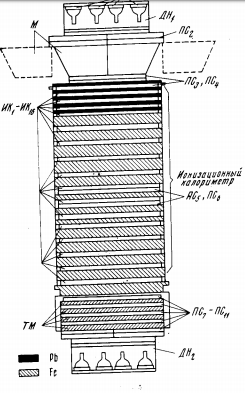
\includegraphics[width=70mm]{pictures/IK15.PNG}
	}
	\caption{Схематическое изображение ИК-15}
	\label{picIK15}
\end{figure}
Для станции <<Протон-4>> телескоп СЭЗ-14 был заменён на ионизационный калориметр ИК-15 (рис. \ref{picIK15}). С двух противоположных концов ИК-15 расположены окна детекторов направлений, каждый из которых состоит из 16 черенковских счётчиков, общая рабочая площадь которых составляет около $3000~см^2$. Выделение частиц в выбранном телесном угле осуществлялось путём отбора совпадений электрических сигналов от одного из детекторов направления с сигналами пропорциональных счётчиков.
\subsection{Спутники серии <<Космос>>}
Серия <<Космос>> состоит более чем из 2,5 тысяч космических аппаратов. На некоторых из них были установлены приборы НИИЯФ МГУ для исследования околоземной радиации и космических лучей. 
В рамках данного литературного обзора интересно рассмотреть несколько ИСЗ, в составе аппаратуры которых присутствовали черенковские детекторы. 

Спутник <<Космос-900>> был запущен в 1977 году, проработал более 3 лет. Среди приборов был черенковский детектор, сконструированный Е.В.\,Горчаковым ~\cite{KOSMOS900}.
Радиатор выглядел как цилиндр из плексигласа с диаметром 30 см. 
Для своего времени детектор обладал огромным геометрическим фактором ($7500~см^2\,\cdot\, стер$).
Из-за большого геометрического фактора прибор обладал большой чувствительностью к относительно небольшим потокам высокоэнергичных электронов радиационных поясов.
С помощью этого прибора были обнаружены  узкие электронные пояса с $E_e\geq15~МэВ$ между внутренним и внешним радиационными поясами во время геомагнитных возмущений. Пояса существуют в течение нескольких дней, затем исчезают. События происходят на фазе восстановления геомагнитной бури и коррелируют с увеличением скорости солнечного ветра.
\begin{figure}[th]
	\noindent\centering{
		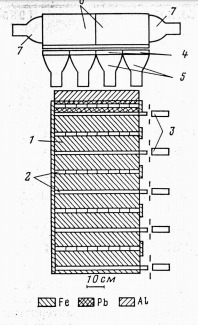
\includegraphics[width=70mm]{pictures/SOKOL.PNG}
	}
	\caption{Схематическое изображение прибора <<Сокол>>}
	\label{picSOKOL}
\end{figure}
В в 1984 и 1986 гг. соответственно состоялись запуски спутников <<Космос-1543>> и <<Космос-1713>>. Для проведения эксперимента по изучению химического состава и спектра частиц ПКИ был разработан прибор <<Cокол>> (рис. \ref{picSOKOL}). 
Вес аппаратуры – 2500 кг, орбита спутников находилась на высоте около 300 км. 
Спутник был ориентирован так, чтобы продольная ось прибора была ориентирована вдоль земной оси <<зенит – надир>>. <<Сокол>> состоял из трёх блоков: ионизационного калориметра ИК и двух блоков измерения заряда ДЗ-1 и ДЗ-2. Детекторы заряда служили также в качестве детекторов направления. ДЗ-1 состоял из 11 независимых черенковских счётчиков, определяющих заряд первичных лёгких ядер ($1\geq Z\geq 6$), а ДЗ-2 состоял из 4 счётчиков, регистрирующих тяжёлые ядра ($6\geq Z\geq 50$). Радиаторы детекторов были сделаны из плексигласа и были почернены с торцов, в которые входили частицы.
Главной особенностью прибора была возможность визуализации картины прохождения частицы через вещества детекторов.
На ИСЗ <<Космос-1713>> прибор <<Сокол>> был несколько модернизирован. В нём был расширен диапазон регистрации зарядов блоком ДЗ-1 и были изменены поглотители калориметра. Управляющий сигнал на регистрацию события вырабатывался по схеме совпадения трёх сигналов: сигнала в ДЗ-1, энерговыделения в ИК и энерговыделения в первых $m$ рядах поглотителя.
\section{Зарубежные черенковские детекторы в космосе}
В этом разделе выбраны два наиболее значимых прибора для ознакомления. Разумеется, список гораздо больше (например, работы \cite{Shuttle}, \cite{ESRO2},\cite{ISEE3}, однако в рамках литературного обзора остановимся на двух интересных примерах.
\subsection{Телескоп на борту Space Shuttle STS-57}
\begin{figure}
	\noindent\centering{
		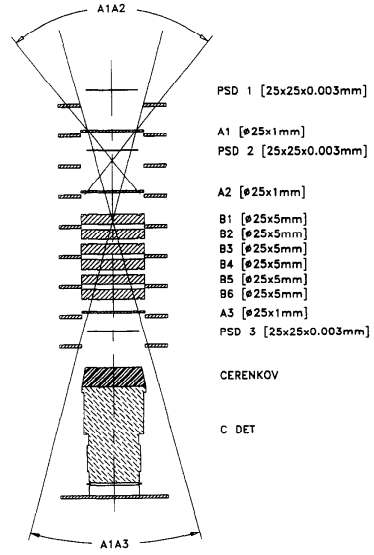
\includegraphics[width=70mm]{pictures/ShuttleSTS57.PNG}
	}
	\caption{Схематическое изображение телескопа на STS-57}
	\label{figSTS57}
\end{figure}
Согласно \cite{ShuttleSTS57}, в 1994 году были произведены измерения потоков заряженных частиц ГКЛ в рамках программы SPACEHAB 2 на борту Space Shuttle во время полета STS-57. При измерениях использовался твердотельный телескоп, (см. рис. \ref{figSTS57}), который состоял из 6 слоёв полупроводниковых кремниевых детекторов (А1–А3 и B1–B3) и сапфирового черенковского детектора, напрямую выходящего к ФЭУ. Весь телескоп был окружён мантией из сцинтилляционного вещества, находящегося в оптическом контакте с 4 фотоумножителями. Сигнал с противоположных ФЭУ складывался, и таким образом получалось два независимых сигнала D1 и D2 от этого детектора. Каждый из детекторов A1–B4 был обеспечен АЦП с разрешением в 4096 каналов, а частота счётов детекторов фиксировалась каждые 10 секунд. Телескоп был размещён в середине шаттла и зафиксирован так, чтобы его ось совпадала с осью самого шаттла. Черенковский сапфировый детектор имел порог регистрации около 200 МэВ/нуклон, однако синтетический сапфир также обладал сцинтилляционными свойствами, и детектор срабатывал как от черенковских, так и от сцинтилляционных вспышек. Также существовала описанная выше проблема обратного тока, в связи с чем частицы, которые распознавались как <<протоны>>, могли быть, например, пионами или каонами. 

\subsection{Эксперимент MARIE на борту Mars Odyssey}
В 2001 году был запущен аппарат Mars Odyssey, который действует на орбите Марса до сих пор. На его борту находится прибор MARIE (Martian radiation environment experiment) \cite{MARIE}, предназначенный для измерения фоновой радиационной обстановки, связанной с солнечными протонами и потоками ГКЛ в диапазоне энергий 20-500 МэВ/нуклон. 
\begin{figure}
	\noindent\centering{
		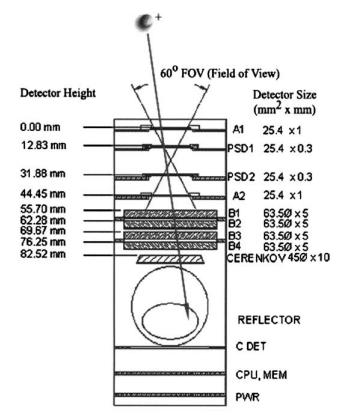
\includegraphics[width=.9\textwidth]{pictures/MARIE.PNG}
	}
	\caption{Схематическое изображение аппарата MARIE}
	\label{figMARIE}
\end{figure}
Внутри MARIE (рис. \ref{figMARIE}) в стеке расположены девять детекторов, действующих как телескоп. Полупроводниковые детекторы A1--A2 и B1--B4 являются основными идентификаторами частиц. Частицы с достаточной энергией проходят через все слои детекторов, однако некоторые частицы останавливаются в детекторных слоях.  Заряд и энергия таких частиц могут быть определены по выделенной в слоях детектора энергии и глубине проникновения. Если частица проходит в пределах конуса с углом раствора в 60 градусов и её энергии достаточно, чтобы пройти через слои A1 и A2 (каждый толщиной в 1 мм, также между ними помещены две пластины позиционно-чувствительных детекторов толщиной 300 мкм), то такое событие считается совпадением. В таком случае все платы детекторов опрашиваются CPU, и данные для этого события записываются. Для каждого слоя детектора записывается индивидуальное выделенное количество энергии. С помощью PSD определяется и записывается трек частицы в детекторе. За A2 расположены четыре Si(Li)-детекторы толщиной 5 мм, с помощью которых проводятся измерения с высоким разрешением. За ними расположен черенковский детектор С, осуществляющий отбор частиц с энергией больше 500 МэВ/нуклон. Кроме того, он также выполняет функцию детектора направления. 
Черенковское излучение из радиатора с помощью зеркала отражается в ФЭУ. Преимущество этой конструкции перед другими состоит в том, что  после радиатора можно поставить ещё слои детекторов.

\chapter{Экспериментальная часть работы}
Эта глава посвящена созданию черенковского детектора релятивистских электронов. Описан процесс создания прибора, его характеристики. Проведено несколько экспериментов с источниками радиоактивного излучения. Работа велась под руководством И.А.~Рубинштейна.
\section{Функциональный облик прибора}
\begin{figure}[t]
	\hfill
	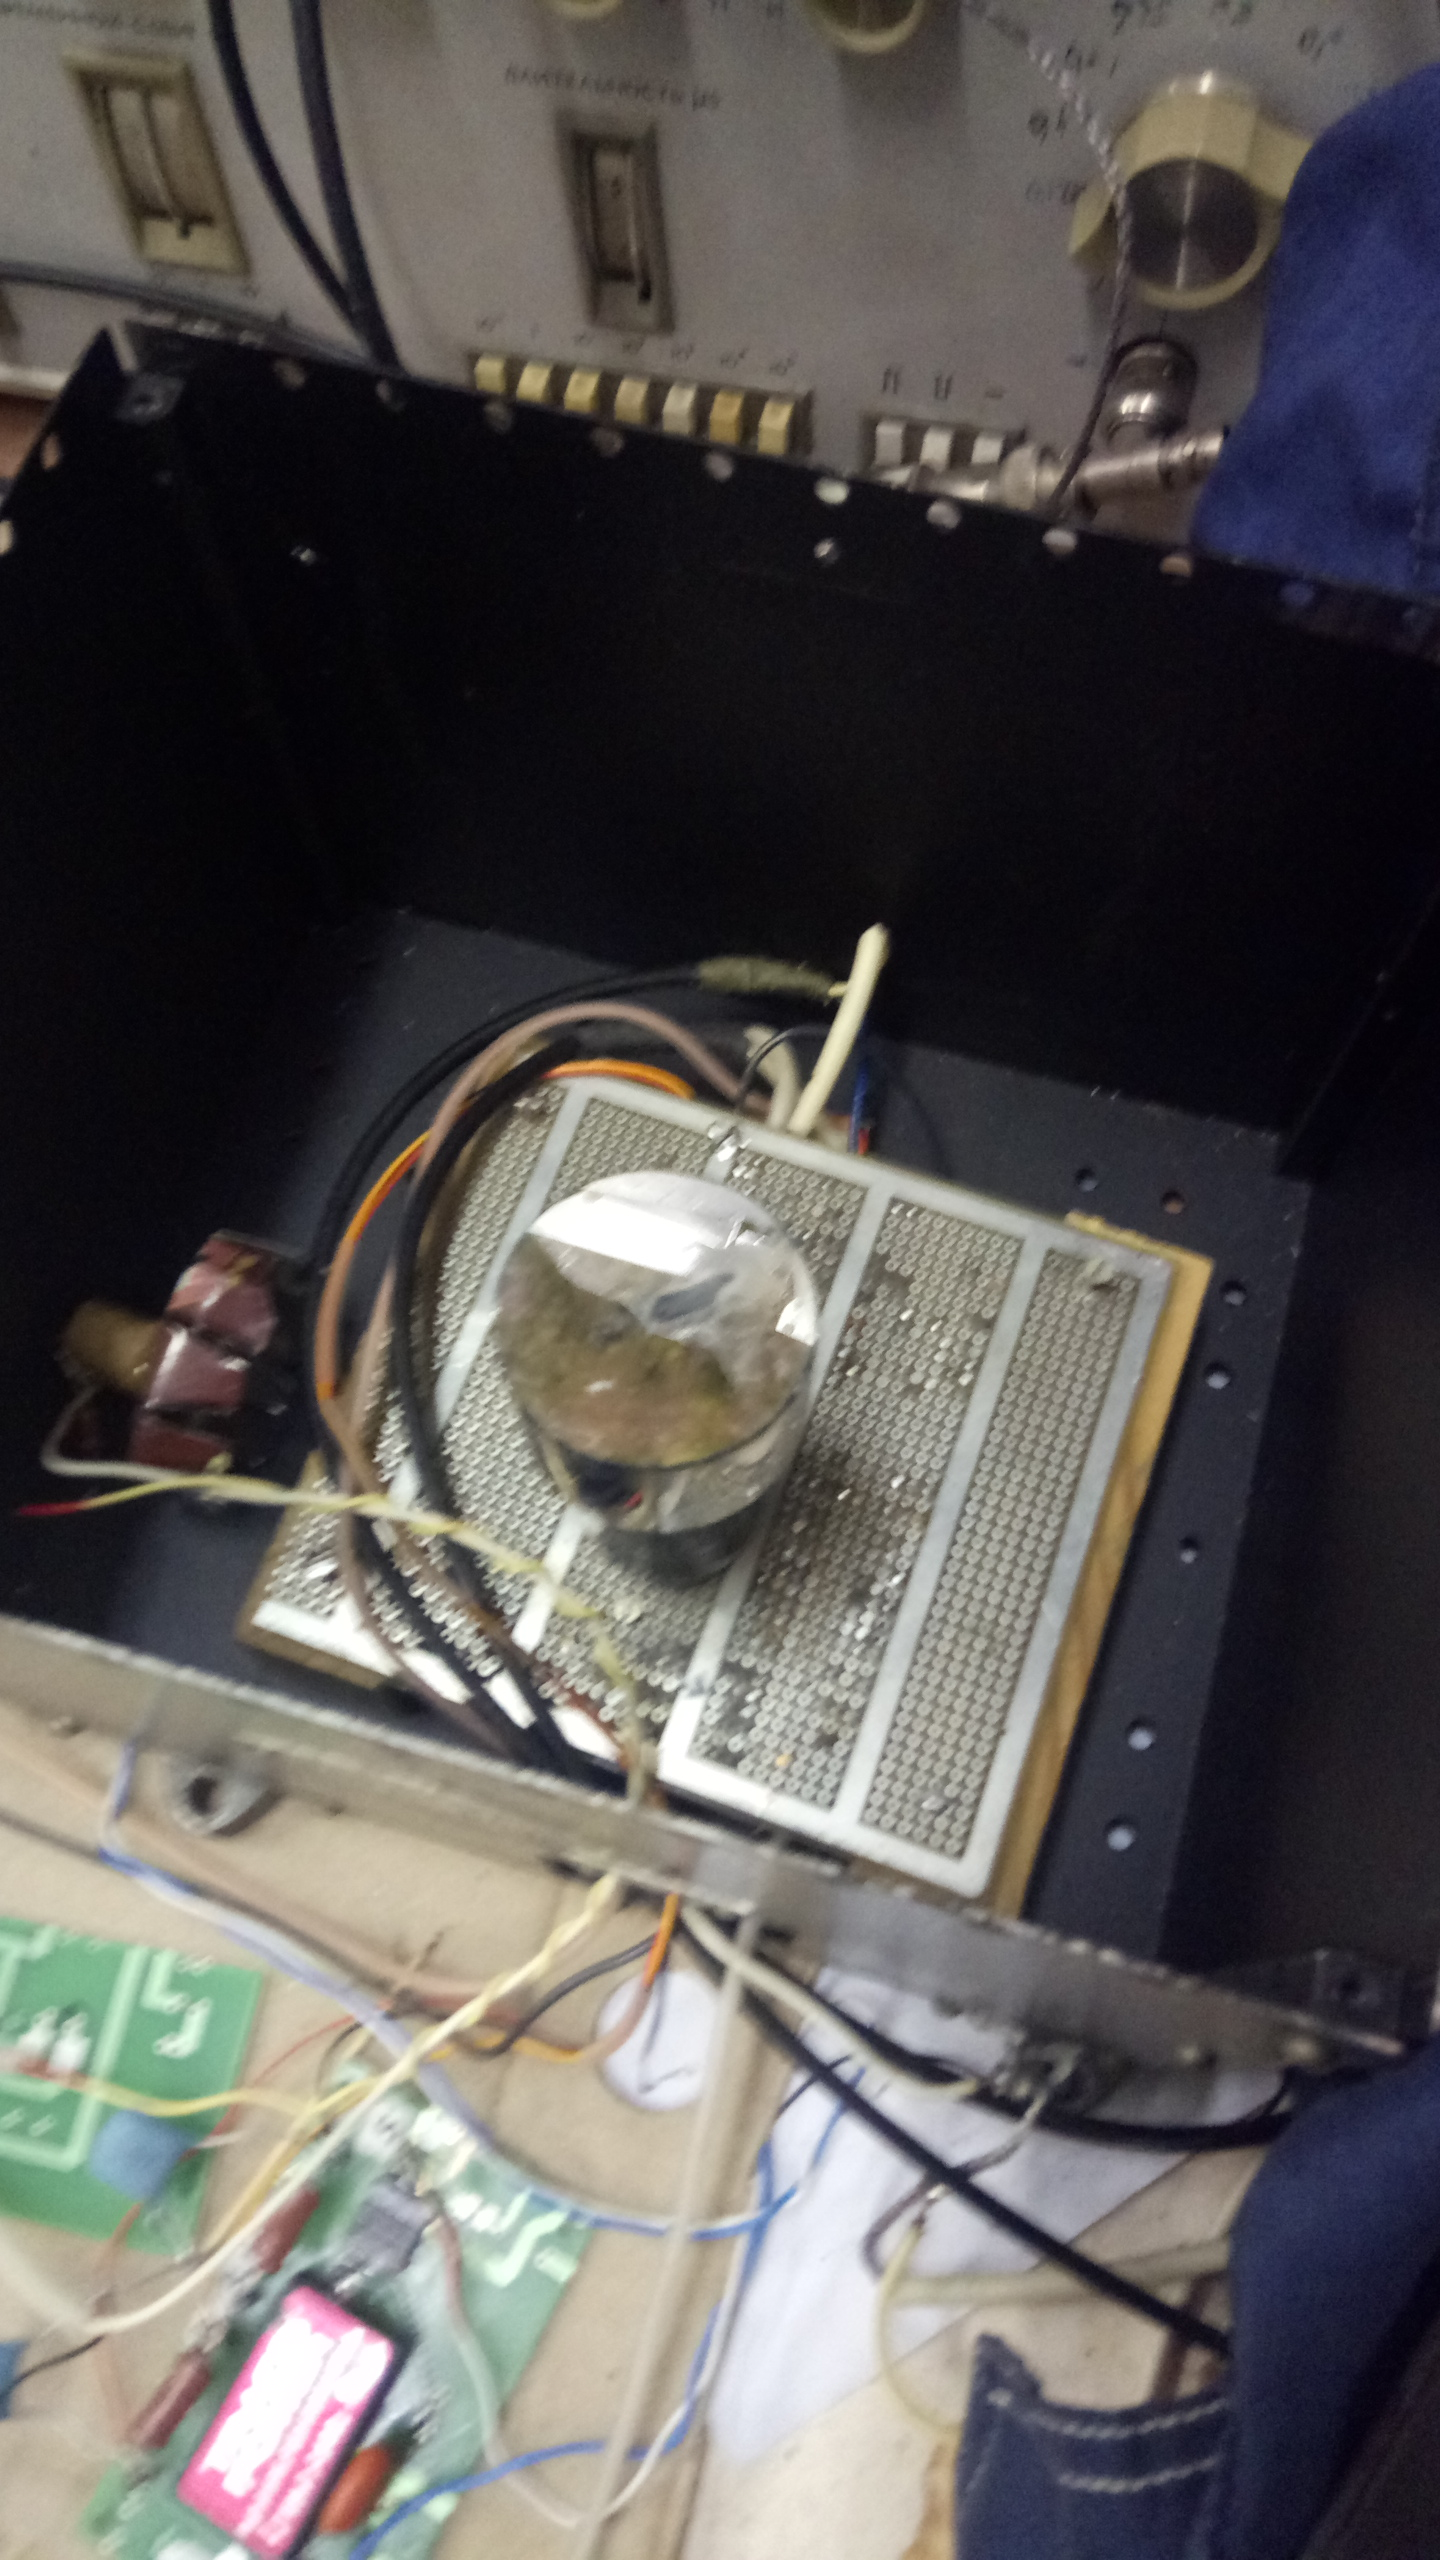
\includegraphics[width=70mm]{pictures/pribor.jpg}
	\hfill
	\caption{Внешний вид прибора}
	\label{pribor}
\end{figure}
В состав прибора входят следующие элементы: радиатор, фотоэлектронный умножитель, электронная плата. При попадании в радиатор частицы с высокой энергией, возникает вспышка черенковского света. Часть света собирается и поступает во входное окно ФЭУ, где в результате каскадного процесса фотоэффекта при приложенной к катоду и аноду большой разности потенциалов, на анод приходит отрицательный заряд. Заряд поступает на зарядовочувствительный усилитель (ЗЧУ), откуда импульс поступает на вход младшего усилителя (ОУ). С выхода этого усилителя импульсы поступают на плату АЦП, которая подключена к персональному компьютеру. Программа, разработанная специально для этой платы, набирает статистику импульсов. Теперь подробнее о каждом из элементов:
\begin{itemize}
	\item Радиатор. Роль радиатора в приборе играет кристалл кварцевого стекла марки КУ-1 (кварц ультрафиолетовый). Кристалл состоит из двух фигур: цилиндра диаметром 40 мм и высотой 25 мм и усечённого конуса (больший диаметр 40 мм, меньший диаметр 28 мм, высота 8 мм). Радиатор покрыт слоем высокочистого (концентрация примесей меньше $0,001$) полированного алюминия. Ниже (табл. \ref{tab:optical}) представлена зависимость оптического показателя преломления от длины волны в оптическом и ближнем ультрафиолетовом диапазонах. 
\begin{table}[bh!]
		\caption{\label{tab:optical}Зависимость показателя преломления КУ-1 от длины волны $n(\lambda)$ (ГОСТ 15130-86)}
		\begin{center}
		\begin{tabular}{|c|c|}
		\hline
		Длина волны $\lambda$, нм & Показатель преломления $n$ \\
		\hline
		184.89&1,575131 \\
		190&1,5657 \\
		190 &1,5657 \\
		193&1,560841\\
		193,40&1,560208\\
		194,17&1,559012\\
		200&1,5505\\
		206,20&1,542741\\
		220&1,5285\\
		248,4&1,5086\\
		266&1,4997\\
		308&1,4856\\
		337&1,4792\\
		365,48&1,4748\\
		404,65&1,4696\\
		488&1,4630\\
		532&1,4607\\
		590&1,4585\\
		600&1,458\\
		632,8&1,4570\\
		650&1,455\\
		\hline
		\end{tabular}
		\end{center}
	\end{table} 
Видно, что пороговая скорость частицы должна лежать в пределах $\beta_{min}= 1/n = 0,637 \div 0,690$. Учитывая, что $E=mc^2+T = mc^2/\sqrt{1-\beta^2}$, получаем, что для данного стекла пороговые энергии электрона $T_{пор}$, мюона и протона есть соответственно 0,2, 35 и 310 МэВ (приблизительно).
	\item Фотоумножитель Hamamatsu Photonics R7111Q. Технические характеристики ФЭУ указаны в официальной документации \cite{Hamamatsu}. Необходимо отметить, что Q  в названии обозначает кварцевое входное окно для большей квантовой чувствительности к ультрафиолетовому излучению. Спектральная область высокой чувствительности лежит в пределах 200--700 нм. 
	\item Электронная плата. Плата содержит в себе делители напряжения для динодов ФЭУ, два усилителя, а также источник высоковольтного питания EMCO CA20N и систему управления для него. Рабочее напряжение платы +22\dots26 В. 
\end{itemize}

\section{Подбор оптимального напряжения}
Диноды и анод изготовлены из металла, покрытого плёнкой вещества с малой работой выхода электронов. Это нужно для увеличения коэффициента вторичной эмиссии $\sigma$, под которым обычно подразумевается среднее число вторичных электронов, выбиваемых первичным электроном. Если $\sigma$ "--- коэффициент вторичной эмиссиии на каждом диноде, то среднее значение коэффициента усиления ФЭУ есть 
\begin{equation}
	\kappa = q\sigma^n, 
\end{equation}
где $0 <q <1$ "--- множитель, учитывающий неполное собирание электронов с фотокатода на первый динод, а $n$ "--- число динодов. Для PMT R7111Q $\kappa= ~2.0\cdot10^6$ при напряжении $U = 1250 В$, указанном заводом-производителем в качестве номинального. Величина коэффициента вторичной эмиссии также зависит и от напряжения питания ФЭУ: $\sigma$ быстро возрастает при росте $U$. Зависимость в области больших напряжений может быть представлена в виде
\begin{equation}
	\sigma = AUe^{-U/U_0},
\end{equation}
где $A, U_0$ "--- постоянные, определяемые свойствами материала поверхности динодов (в т.ч. работой выхода электронов с плёнки), а $U$ -- ускоряющее напряжение между двумя соседними динодами (будем считать, что все делители напряжения одинаковы, и потенциалы распределены равномерно). Таким образом, коэффициент усиления $\kappa$ представим в виде:
\begin{equation}
	\kappa = qA^nU^ne^{-nU/U_0} 
\end{equation}
При полном затемнении и холостой работе ФЭУ (без источников световых вспышек) шумы ФЭУ имеют вид отдельных малых импульсов порядка нескольких сотен милливольт, вызванных вылетом единичных электронов с поверхности фотокатода под действием термоэлектронной эмиссии. Они не зависят от приложенного напряжения и определяются температурой фотослоя. 
Однако при высоком напряжении и большом коэффициенте усиления возникает резкое возрастание шумов ФЭУ. Наряду с тепловыми шумами в ФЭУ наблюдается возникновение шумов, зависящих от напряжения и вызванных автоэлектронной эмиссией или оптической обратной связью.
\begin{figure}[th]
	\noindent\centering{
		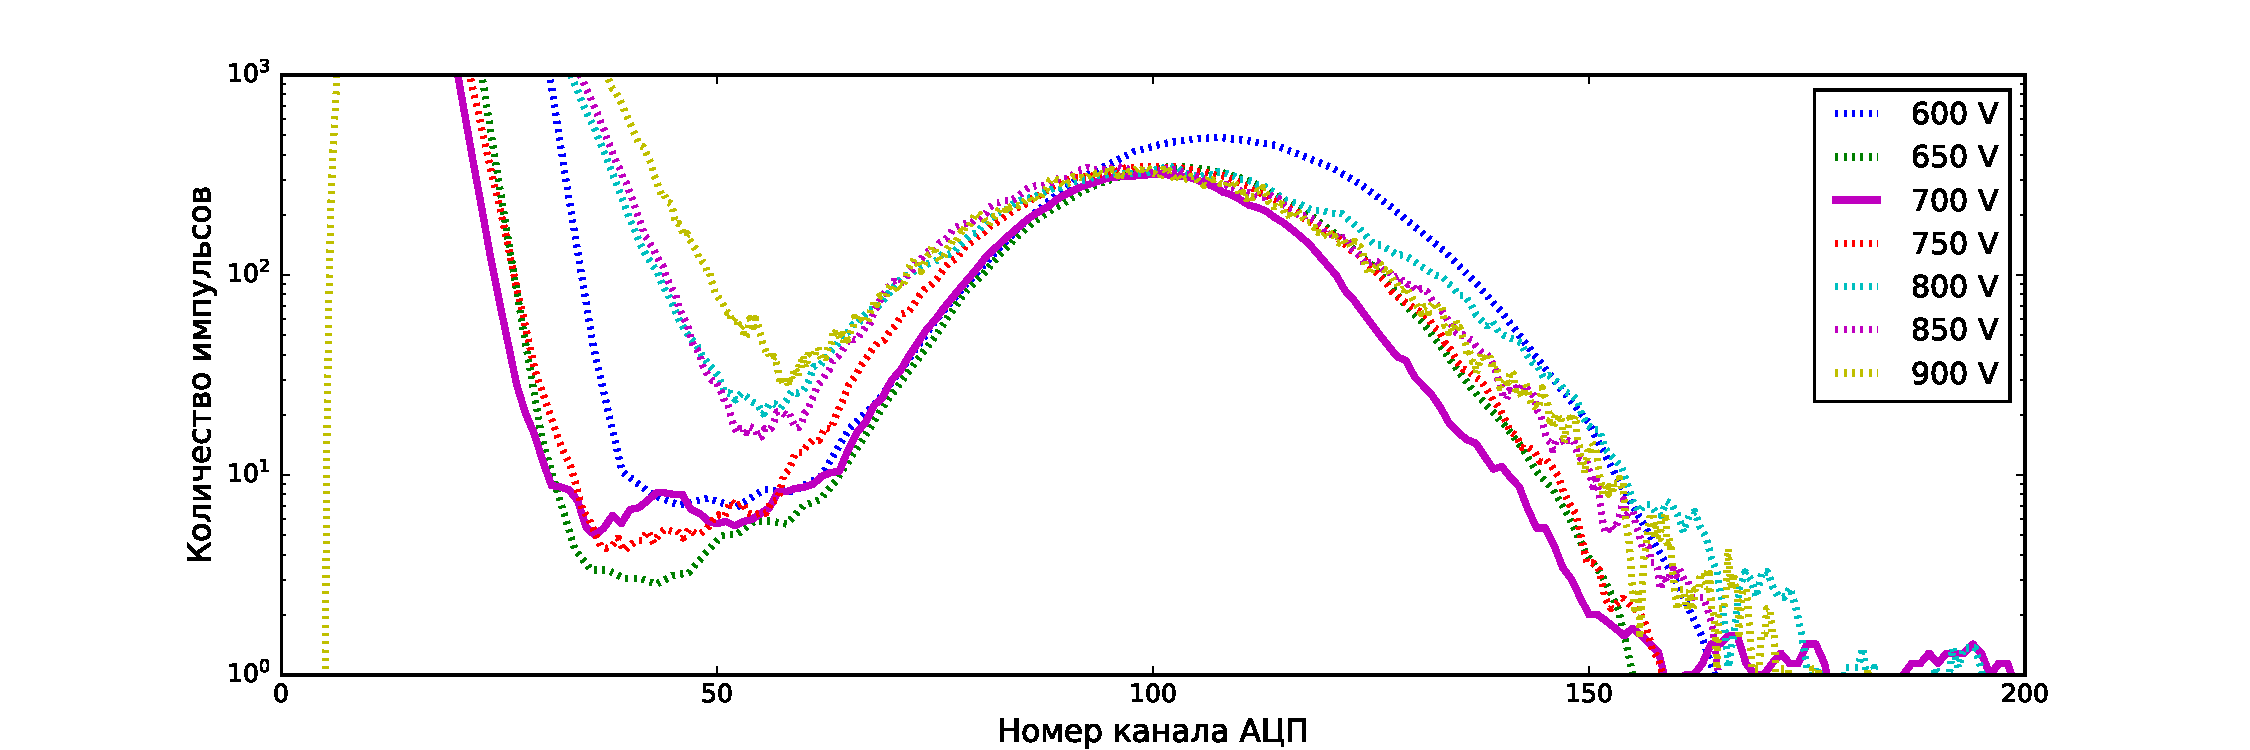
\includegraphics[width=170mm]{pictures/VoltageModes.pdf}
	}
	\caption{Отнормированные сглаженные <<спектры>> c АЦП для импульсов на светодиоде}
	\label{UVlight}
\end{figure}

Возникает необходимость найти оптимальный режим напряжения, который обеспечивает максимальный коэффициент усиления ФЭУ, но при котором шумы ещё слабо зависят от питания. Система управления высоковольтным питанием позволяет менять напряжение в диапазоне 0--1300 В. Для подбора оптимального режима использовалась следующая схема эксперимента: к генератору прямоугольных импульсов был подключён ультрафиолетовый светодиод, светящий в торец радиатора. Световые импульсы имитировали черенковские вспышки внутри радиатора и создавали импульсы на аноде ФЭУ. После каскада усилителей импульсы поступали на АЦП, который распределял события по каналам. Типичный <<спектр>> такого наблюдения экспоненциально спадал на младших каналах (тепловые шумы) и имел явно выраженный пик (импульсы от светодиода одной амплитуды). Напряжение увеличивалось шагами по 50-100 В. При разности потенциалов больше 700 В проявились дополнительные шумы. На приведённом рисунке \ref{UVlight} <<спектры>> отнормированы по обеим осям (т.\,е. приведены к одной координате и значениям максимумов) и сглажены методом скользящего среднего. Оптимальный режим напряжения "--- 700 В "--- показан сплошной пурпурной линией. Как видно, при б\'oльшем напряжении экспоненциальный хвост начинает сдвигаться правее, что говорит о том, что проявляются шумы, вызванные автоэлектронной эмиссией. 

\section{Первые тесты на радиоактивных изотопах}
После выбора оптимального режима напряжения были осуществлены испытания на радиоактивных изотопах, а также измерение естественного радиационного фона (рис. \ref{figNoise}). Каждая экспозиция с набором статистики длилась 90 минут. Во избежание перегрузки памяти АЦП регистрацией шумовых импульсов от ФЭУ был предварительно выставлен порог. Регистрировалась статистика импульсов висмута и двух препаратов стронция с разной активностью. Полученные спектры были зашумлены ложными срабатываниями ФЭУ, а также естественным фоном от космических лучей. Для выделения сколько-либо значимых результатов применялся грубый метод: из полученного спектра от источника вычитался спектр радиационного фона. Это привело к большому количеству артефактов на спектрах, однако демонстрирует правильное функционирование прибора. 
\begin{figure}
	\noindent\centering{
		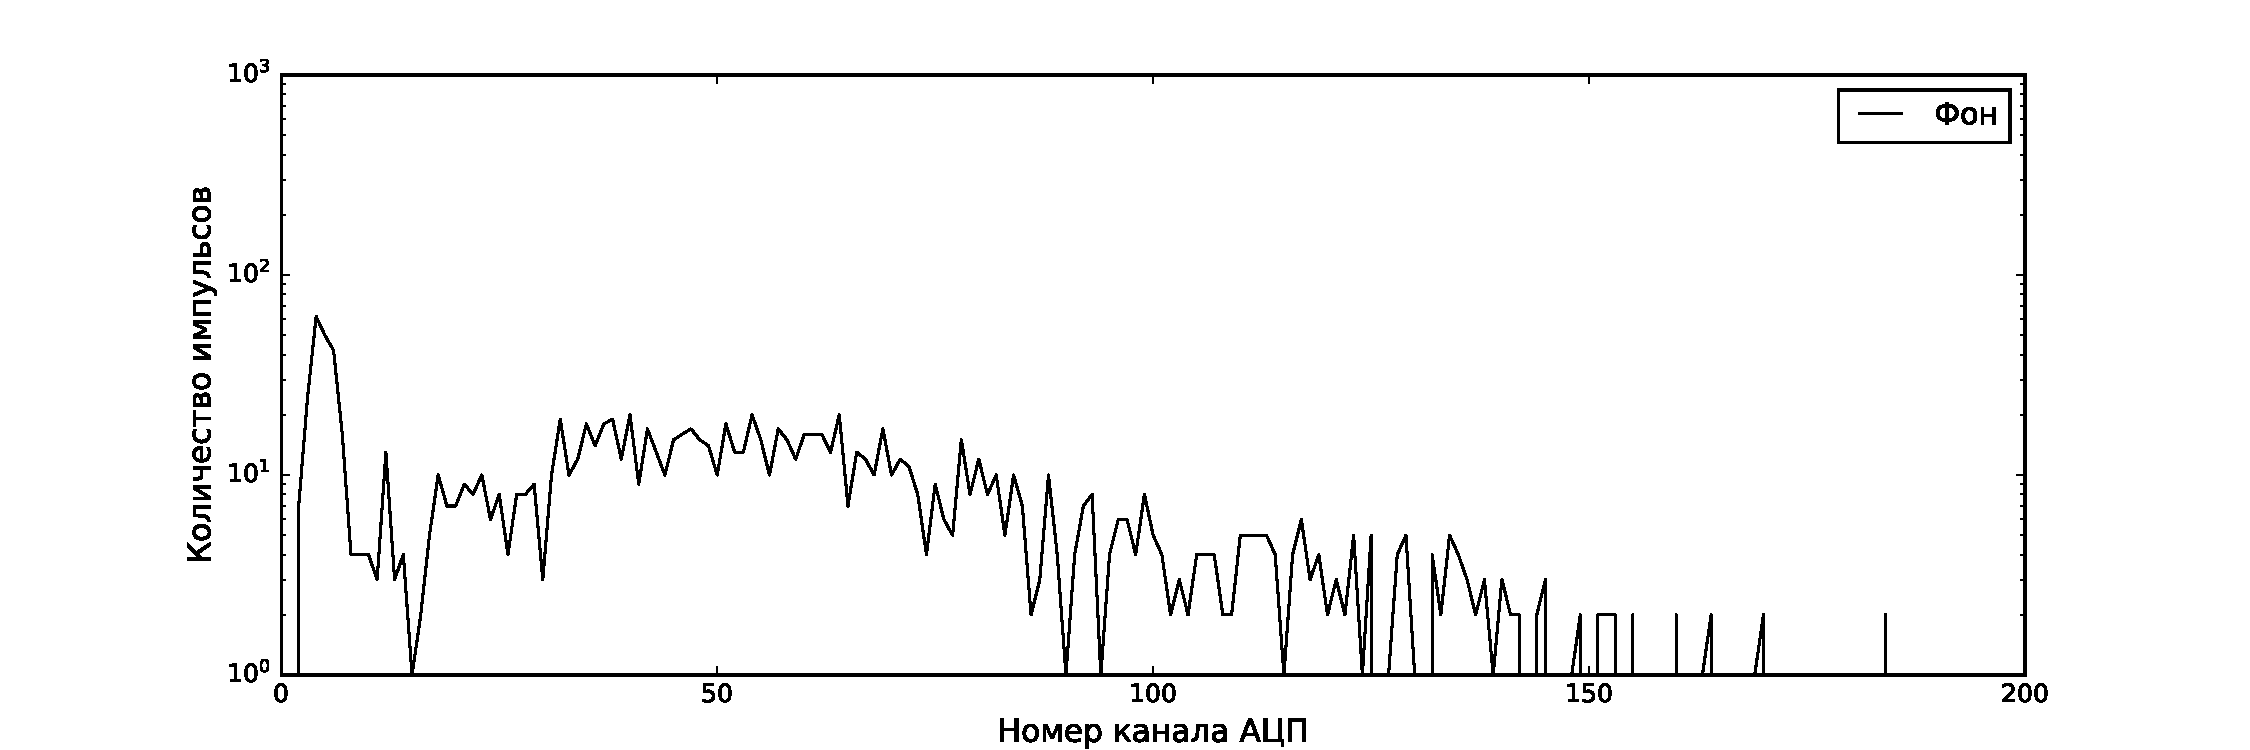
\includegraphics[width=.9\textwidth]{pictures/Noise.pdf}
	}
	\caption{Естественный радиационный фон в полуторачасовой экспозиции}
	\label{figNoise}
\end{figure}
\begin{figure}
	\noindent\centering{
		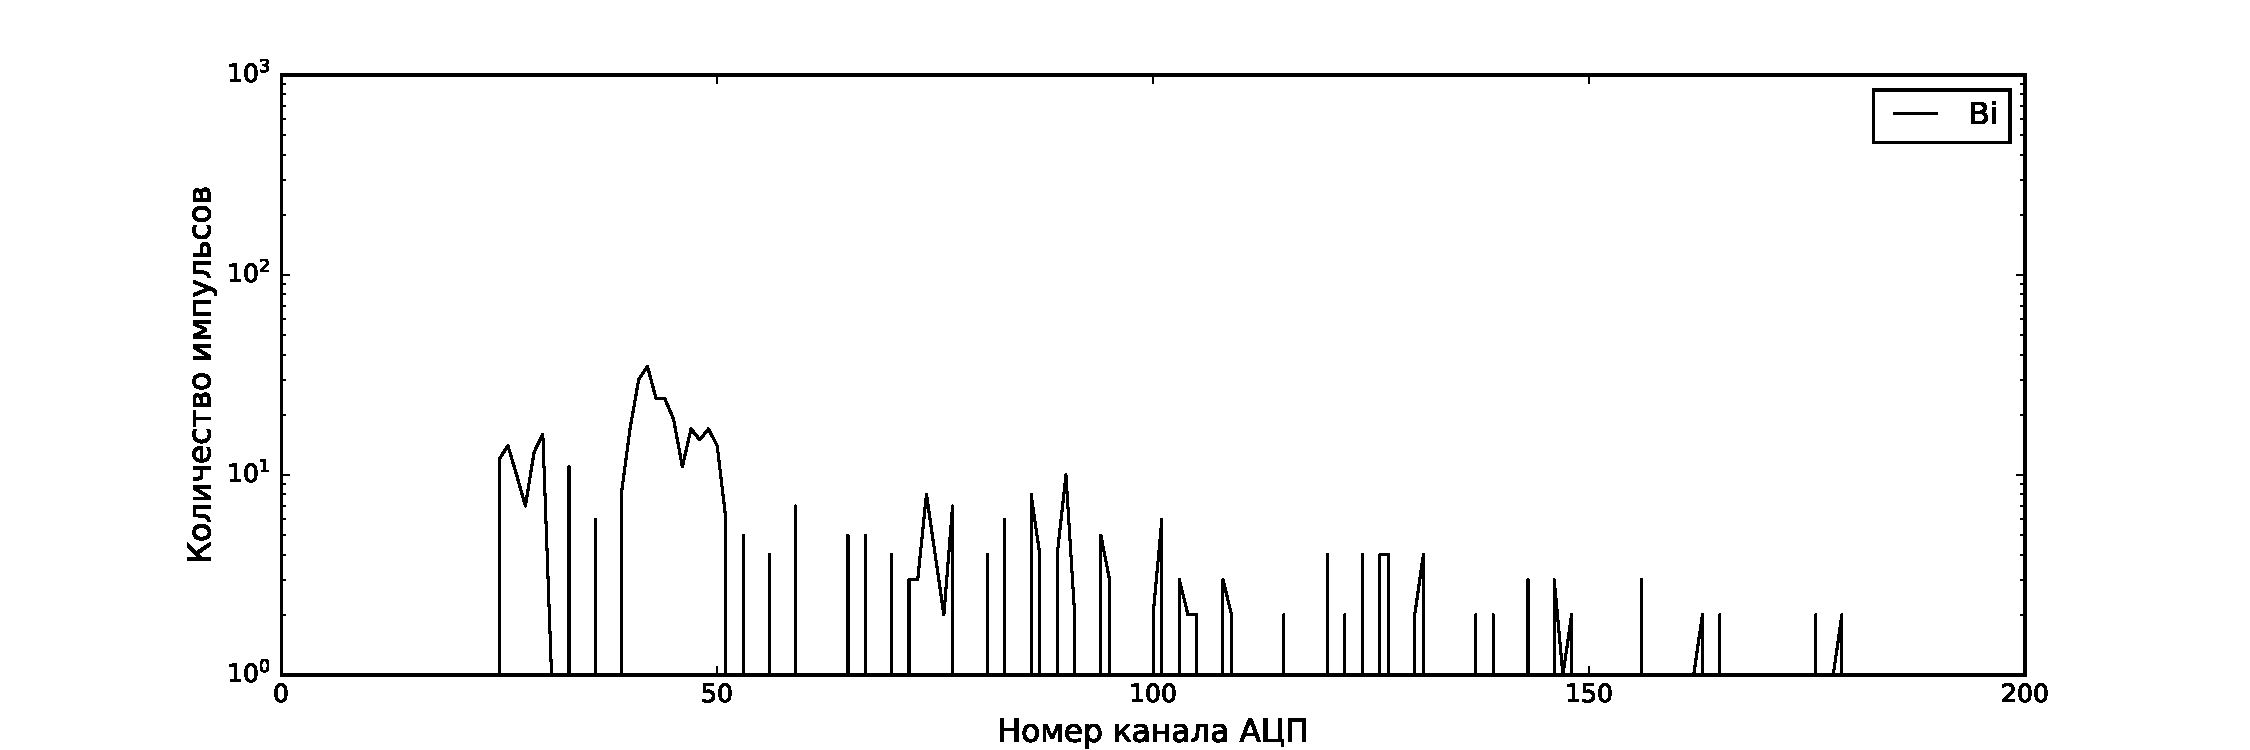
\includegraphics[width=.9\textwidth]{pictures/Bi90.pdf}
	}
	\caption{Статистика импульсов от висмута (без фона)}
	\label{figBi90}
\end{figure}
\begin{figure}
	\noindent\centering{
		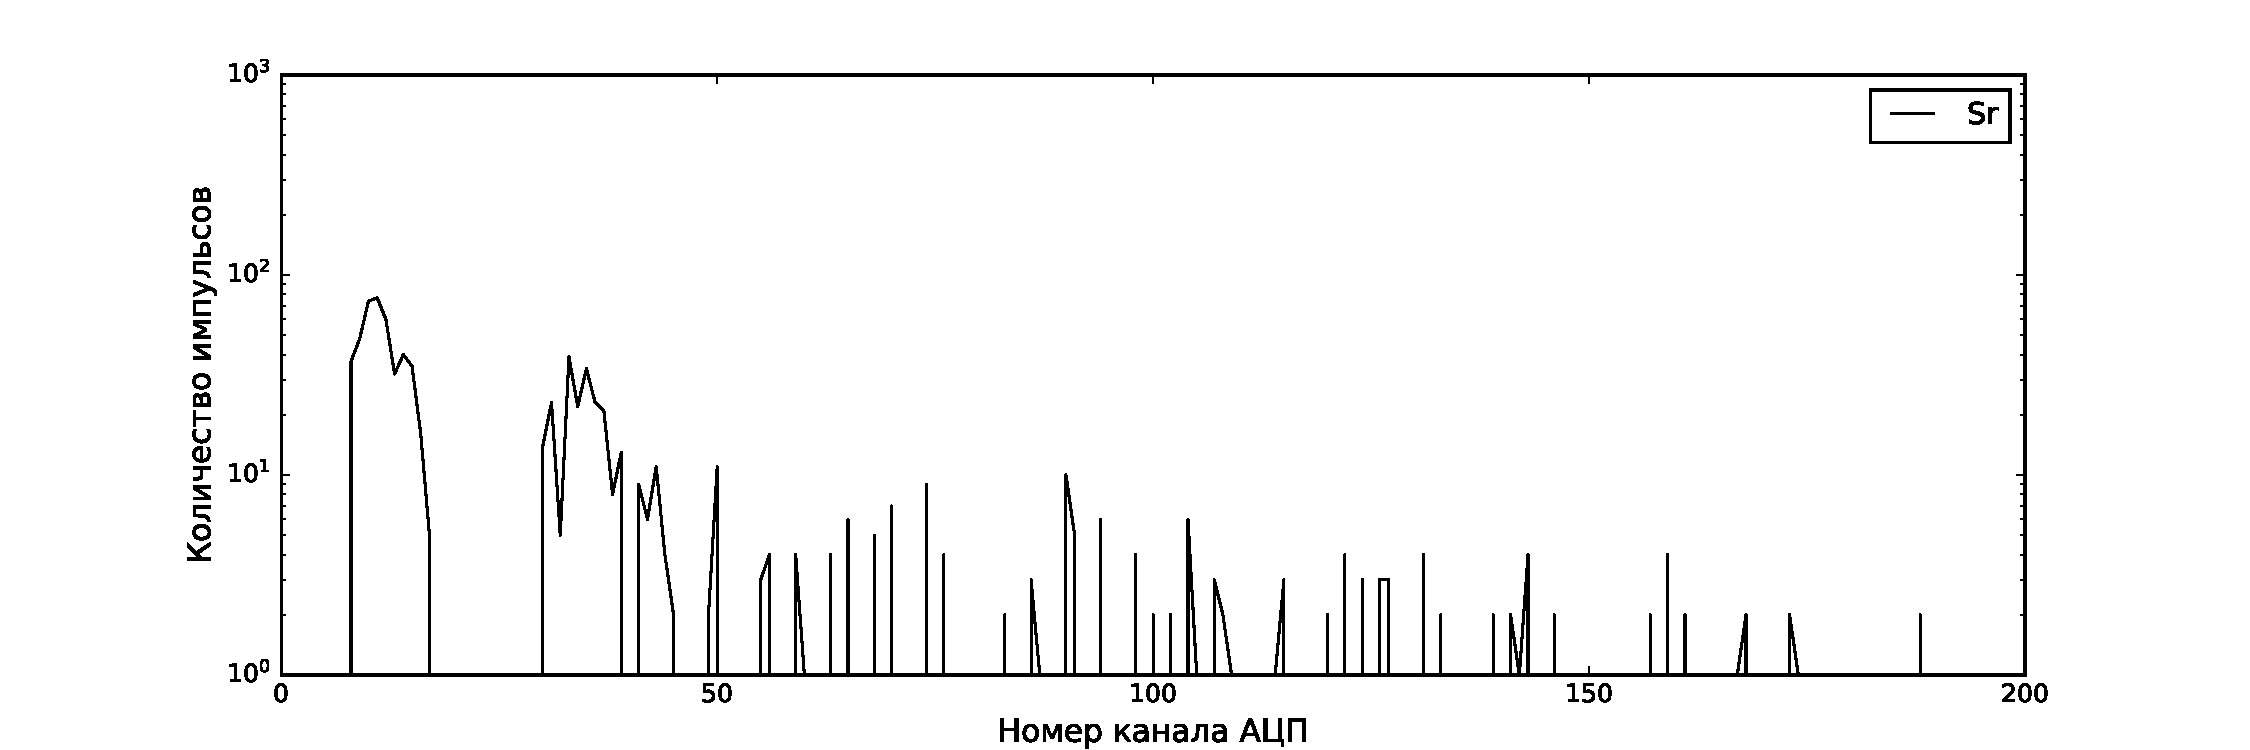
\includegraphics[width=.9\textwidth]{pictures/STR90.pdf}
	}
	\caption{Статистика импульсов от стронция (без фона)}
	\label{figSTR90}
\end{figure}
Разность набранных спектров и шумов демонстрирует, что в каналах 30--50 у обоих препаратов (рис. \ref{figBi90} и \ref{figSTR90}) есть возвышение, превышающее шум интегрально приблизительно на $10^3$ событий.
\chapter{Модельная часть работы}
Параллельно с предыдущими двумя направлениями велась работа по моделированию черенковского детектора с помощью комплекса программ с открытым исходным кодом GEANT4. Численное моделирование позволяет оценить различные параметры детектора, а также попробовать спрогнозировать его работу при регистрации частиц, кроме электронов. Полная версия программы вместе с полученными данными для обработки лежит на репозитории IT-хостинга GitHub по адресу \url{https://github.com/SanTelva/Cherencov}.

\section{Моделирование работы прибора с помощью комплекса программ GEANT4}
Радиатор детектора в точности был воссоздан с помощью инструментов, которые предлагает GEANT4. За основу был взят пример OpNovice, включающий в себя PhysicsLists для работы с оптикой и с черенковским излучением в частности. Численная модель позволит оценить траектории и пути заряженных частиц (электронов и протонов) в радиаторе, зафиксировать пороги по энергии частиц для возникновения черенковского излучения, представить траектории черенковских фотонов после рождения в среде и отражения от алюминированных стенок. 
\begin{figure}[t]
	\centering{
	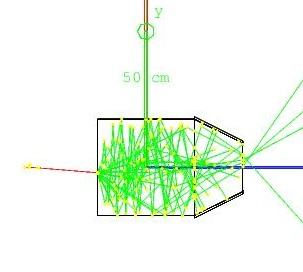
\includegraphics[scale=0.75]{pictures/GEANT/Ris4.jpeg}
	}
	\caption{Одна из визуализаций прохождения электрона через детектор}
	\label{model}	
\end{figure}
\subsection{Количество выделившихся черенковских фотонов}
На данных графиках (рис. \ref{fig:Cercount}---\ref{fig:RegisteredDensity}) можно видеть количество родившихся черенковских фотонов по результатам 10000 симуляций для влетающих в детектор вдоль оси электронов с сеткой по энергии 0,5, 1,0, 1,5, 2,5, 6,0, 8,0 и 10,0 МэВ, а также распределение зарегистрированных в дальнем торце фотонов. 
\begin{figure}[bh]
\begin{center}
	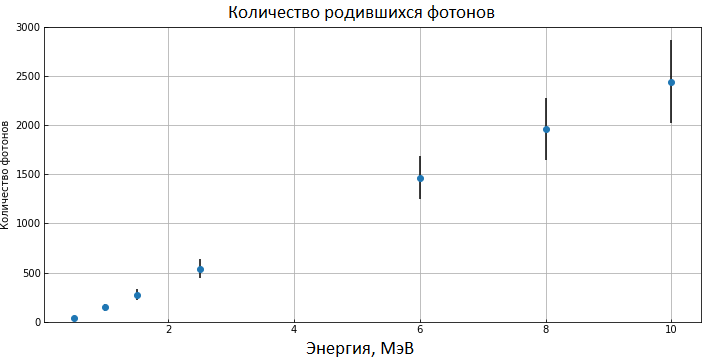
\includegraphics[width=.9\textwidth]{pictures/GEANT/cercount_dependence.png}
	\caption{Количество родившихся фотонов на 1 электрон}
	\label{fig:Cercount}
\end{center}
\end{figure}
\begin{figure}
\begin{center}
	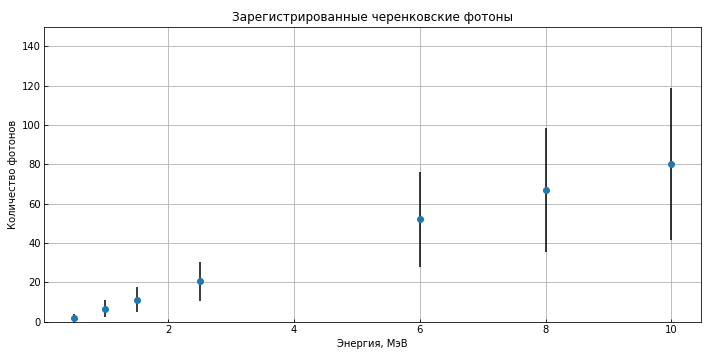
\includegraphics[width=.9\textwidth]{pictures/GEANT/light_dependence.png}
	\caption{Зависимость числа зарегистрированных фотонов на 1 электрон}
	\label{fig:RegisteredLinear}
\end{center}
\end{figure}
\begin{figure}
\begin{center}
	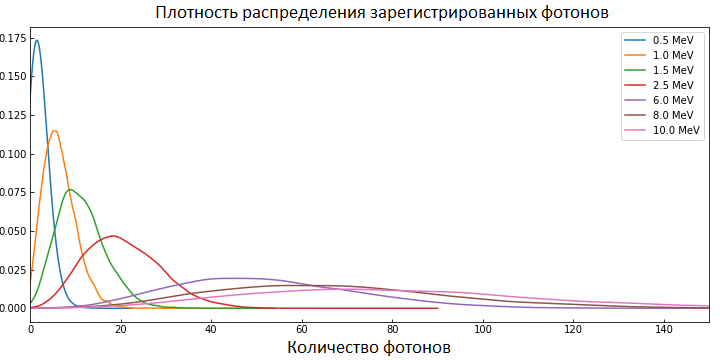
\includegraphics[width=.9\textwidth]{pictures/GEANT/light_density1.png}
	\caption{Плотность распределения зарегистрированных фотонов на 1 электрон}
	\label{fig:RegisteredDensity}
\end{center}
\end{figure}
Количество родившихся фотонов пропорционально энергии первичного электрона (см. рис.~\ref{fig:Cercount} \afterpage{\clearpage}), как и количество зарегистированных (рис.~\ref{fig:RegisteredLinear}\afterpage{\clearpage} ), т.\,е. пролетевших через дальний торец. Доля зарегистрированных, т.\,е. световыход при этом составляет около 4\%.Также, чем больше энергия, тем больше разброс относительно среднего значения, что непременно приведёт к ухудшению энергетического разрешения детектора на больших энергиях. С другой стороны, на фотокатод приходит ничтожно мало фотонов от электронов с энергиями $E_e<2,5$ МэВ, следовательно, эффективность детектора для этих энергий будет невелика. Необходимо отметить, что в модель не закладывались сцинтилляционные свойства кварцевого стекла, присущие почти любому твёрдому веществу, поэтому нет возможности оценить вклад сцинтилляционных фотонов в импульсы, зарегистрированные в приборе. В реальном детекторе их доля должна быть мала, как было указано в ГОСТ 15130-86.

На такой разброс влияют статистический характер рождения черенковских электронов в веществе и сильное их рассеяние от изначального направления из-за большого количества актов столкновения с веществом и малой массы частицы. Модель позволяет проследить траекторию электрона, а также вычислить её длину и глубину проникновения в радиатор.
\begin{figure}[th!]
\begin{center}
	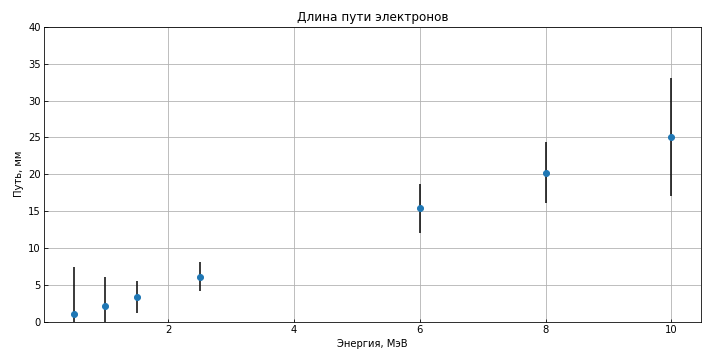
\includegraphics[width=.9\textwidth]{pictures/GEANT/length_dependence.png}
	\caption{Зависимость длины пути электрона от энергии}
	\label{pic:length}
\end{center}
\end{figure}

\begin{figure}[th!]
\begin{center}
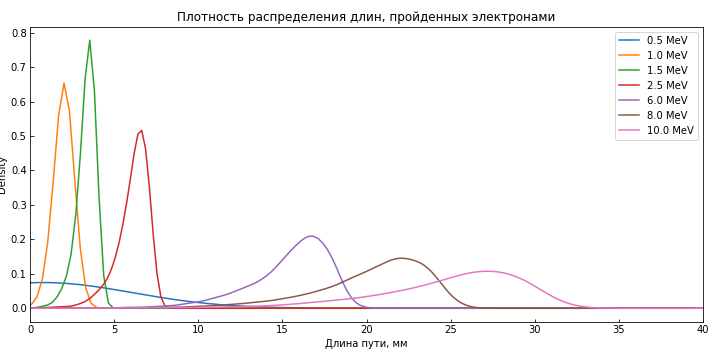
\includegraphics[width=.9\textwidth]{pictures/GEANT/length_density.png}
\caption{Плотность распределения длин, пройденных электронами в веществе радиатора}
\label{fig:lenght_density}
\end{center}
\end{figure}

\subsection{Изучение спектрометрических свойств}
\begin{figure}[h!]
\begin{center}
	\includegraphics[width=.9\textwidth]{pictures/schemem.png}
	\caption{Схема модифицированного телескопа}
	\label{pic:zhut}
\end{center}
\end{figure}
Из-за большого влияния процессов множественного рассеяния на пролёт электронов возникают большие флуктуации длины трека электрона в веществе, что говорит о том, что использовать прибор для прецизионной спектрометрии электронов опрометчиво. Это подтверждают и экспериментальные данные (рис. \ref{figBi90}, \ref{figSTR90}), из которых можно заключить, что величина ширины пика на половине высоты FWHM порядка $100\%$.~Однако инструментарий для моделирования позволяет подробнее изучить спектрометрические свойства, а также угловое разрешение прибора. Для этого можно модифицировать модель, настроив генератор электронов с равномерным распределением энергий в диапазоне  1--11 МэВ в конусе с углом раствора $35\degree$. Схема модифицированного телескопа приведена на~\ref{pic:zhut} \afterpage{\clearpage} .
К детектору также добавлены три дополнительных полупроводниковых слоя для отслеживания энерговыделения. Таким образом, структура получившегося телескопа такова:
\begin{enumerate}
	\item Кремниевая пластинка толщиной 0.04 мм на расстоянии 25 мм от входного торца радиатора. Далее будет обозначена как $Si_1$.
	\item Кремниевый детектор толщиной 0.5 мм вплотную к входному окну радиатора, далее обозначен как $Si_2$.
	\item Сам черенковский радиатор, далее обозначен как $Si_C$.
	\item Кремниевая пластинка толщиной 0.04 мм вплотную у выхода из радиатора. Обозначена как $Si_3$.
\end{enumerate}
Введённые полупроводниковые детекторы нужны для создания схемы совпадений. Из 100000 разыгранных событий выделяются только те, что вызвали энерговыделение в $Si_1$, $Si_2$, $Si_C$ и не вызвали энерговыделения в $Si_3$, т.\,к. последнее означало бы, что частица не остановилась в радиаторе. Появление сигналов на детекторах $Si_1$, $Si_2$ и $Si_C$ свидетельствует о том, что частица влетела в радиатор. 
Все рождённые частицы можно разделить по энергиям на 4 класса диапазонов одинаковой ширины:
\begin{enumerate}
	\item $F_1$ "--- электроны с первичной энергией 1--3.5 МэВ. Цвет: красный.
	\item $F_2$ "--- электроны с первичной энергией 3.5--6 МэВ. Цвет: синий.
	\item $F_3$ "--- электроны с первичной энергией 6--8.5 МэВ. Цвет: зелёный.
	\item $F_4$ "--- электроны с первичной энергией 8.5--11 МэВ. Цвет: пурпурный.
\end{enumerate}
Для каждого электрона вычислены следующие параметры: энерговыделение в первых трёх слоях детектора (или всех четырёх), количество рождённых в радиаторе черенковских фотонов, длина трека в радиаторе и глубина проникновения. Для указанных параметров построены распределения и корреляционные диаграммы различных пар параметров. 
\begin{figure}[th!]
	\begin{center}
		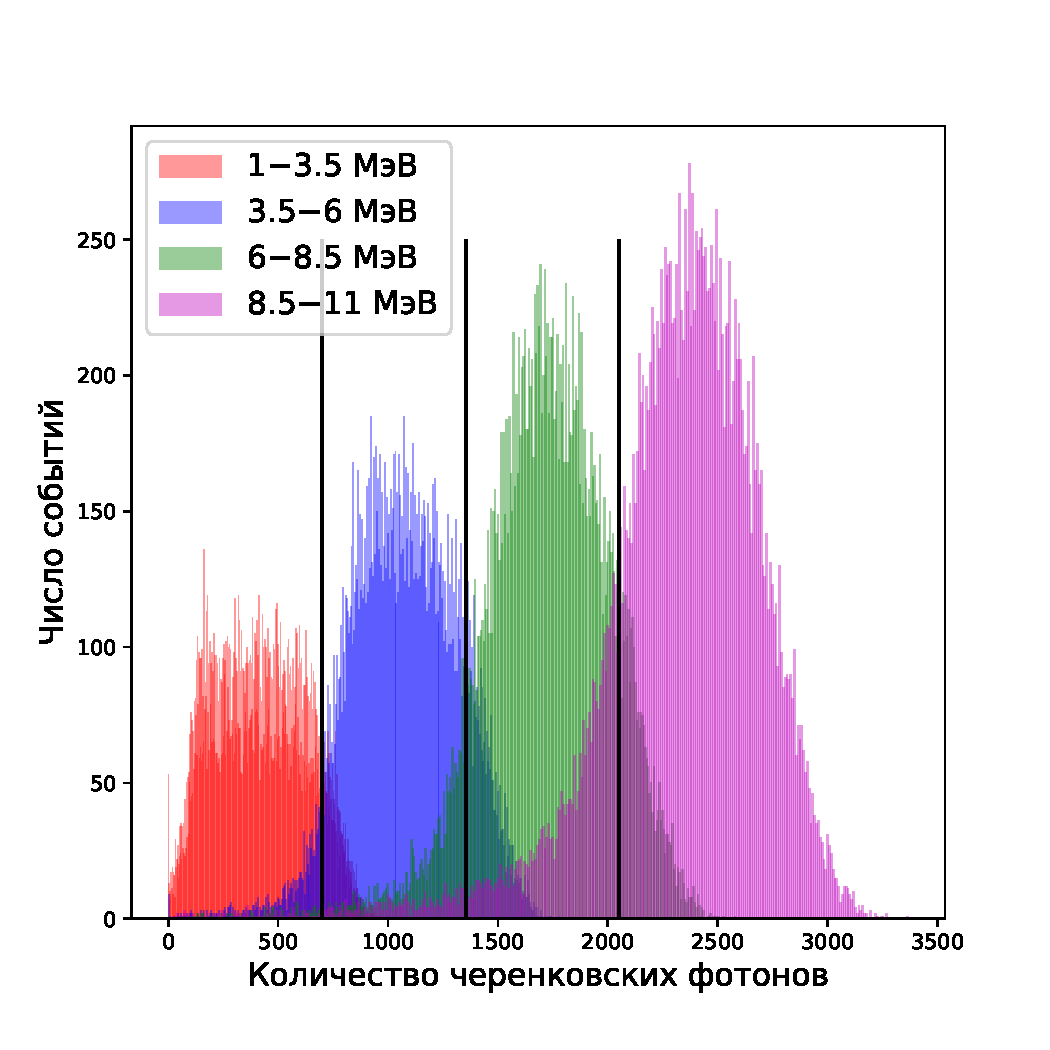
\includegraphics[scale=0.5]{pictures/GEANT/CerenkovPhotonsHist.pdf}
	\caption{Распределение числа рождённых черенковских фотонов}
	\label{fig:CerHist}
	\end{center}
\end{figure}
Из представленной гистограммы~\ref{fig:CerHist}\afterpage{\clearpage} видно, что для каждой группы электронов количество рождённых фотонов нормально распределено. Это даёт возможность по количеству рождённых фотонов грубо оценивать принадлежность к тому или иному энергетическому классу $F_1$--$F_4$.
\begin{figure}[th]
	\begin{center}
		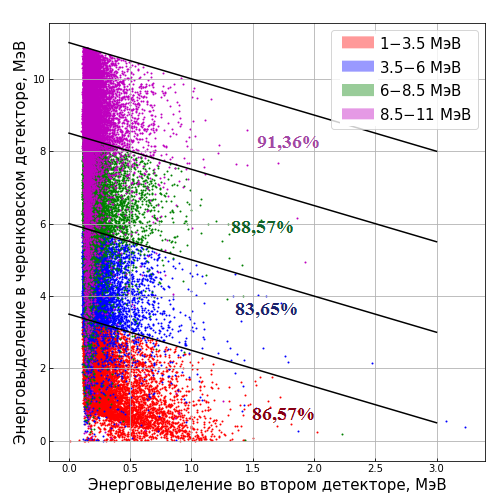
\includegraphics[scale=0.5]{pictures/GEANT/Si2CorrPlotWalls.png}
		\caption{Корреляция энергетических потерь в $Si_C$ и $Si_2$}
		\label{fig:Si2CorrPlot}
	\end{center}
\end{figure}
\begin{figure}[bh]
\begin{center}
	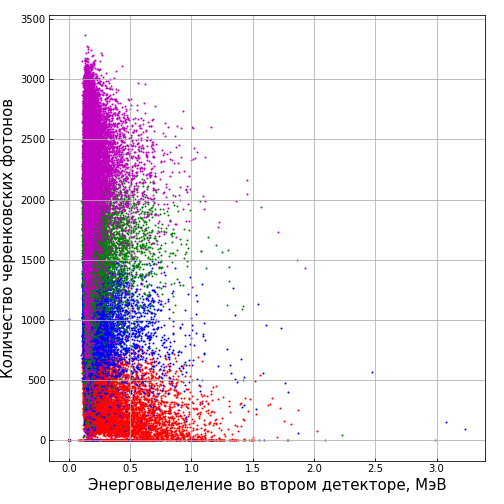
\includegraphics[scale=0.5]{pictures/GEANT/Si2CorrCerCount.png}
	\caption{Корреляция энергетических потерь в $Si_2$ и числа рождённых фотонов}
	\label{fig:Si2CerCorrPlot}
\end{center}
\end{figure}
Подобную классификацию можно провести для корреляции энергетических потерь в $Si_2$ и $Si_C$, которую можно видеть на диаграмме~\ref{fig:Si2CorrPlot} \afterpage{\clearpage}. С помощью прямых $y=3,5-x,~y=6-x,~y=8,5-x$ можно разделить гистограмму на отдельные части, каждая из которых будет включать в себя события из классов $F_1$--$F_4$. Зная, как <<раскрашены>> электроны различных диапазонов, можно посчитать долю правильно обработанных событий (которые были отобраны по схеме совпадений). Эта доля указана на той же гистограмме. 
Диаграмму энергетических потерь $Si_2$ и количества рождённых фотонов~\ref{fig:Si2CerCorrPlot}\afterpage{\clearpage} можно также поделить с помощью линий, только в данном случае придётся усложнить их вид. Точность определения с помощью разбиений параболами указана там же. 

Учитывая приблизительно постоянный коэффициент светосбора рождённых фотонов и приведённую выше эффективность разбиения событий для последующей классификации, можно заключить, что собранный детектор должен обладать спектрометрическими свойствами, позволяющими грубо определять энергию электрона в 4 энергетических диапазонах. 
\chapter*{ВЫВОДЫ}

Выше был изложен доклад по проделанной работе для выпускной работы бакалавра. Для подведения итогов необходимо тезисно изложить полученные результаты по работе над каждым из направлений.

Было изучено большое количество литературы, посвящённой эффекту Вавилова-Черенкова, а также информации о космических аппаратах, включающих в свой состав черенковские детекторы. Эти приборы сыграли большую роль в становлении физики космических лучей, что подтверждают первые космические эксперименты на ИСЗ-3. Впоследствии они выполняли важную функцию внутри телескопов, подавляя проблему обратного тока.
С помощью разработанного Е.\,В. Горчаковым детектора с большим геометрическим фактором было обнаружено такое любопытное явление, как формирование релятивистского электронного пояса в промежутке между внутренним и внешним радиационными поясами на фазе восстановления геомагнитной бури. 

Был разработан функционирующий прибор, регистрирующий частицы, преодолевшие порог черенковского излучения и испытанный на $\beta-$радиоактивных изотопах. Для него подобран оптимальный режим напряжения, обеспечивающий максимальный коэффициент усиления без значительного усиления шумов ФЭУ засчёт автоэлектронной эмиссии. До установления карантинного режима удалось экспериментально установить работоспособность прибора. 

Была описана модель прибора в GEANT4, с помощью которой производилась оценка различных его характеристик. Сделан вывод о том, что в схеме совпадений с дополнительными полупроводниковыми детекторами у телескопа есть возможность его использования в качестве спектрометра.	
\chapter*{ЗАКЛЮЧЕНИЕ}
%\addcontentsline{toc}{chapter}{Заключение}
В заключение необходимо подвести итоги двухлетней работы на кафедре физики космоса. Был освоен спектр навыков и методов для работы с реальными физическими экспериментами. Среди них:
\begin{itemize}
	\item Умение поиска и работы с литературой, посвящённой предмету, среди отечественных источников и зарубежных. 
	\item Всесторонее развитие в области экспериментальной физики.
	\item Базовые навыки работы с электроникой, создание и наладка полноценного прибора. 
	\item Начальное освоение комплекса ПО GEANT4 и его использование для моделирования различных процессов с учётом оптических свойств материала.
	\item Совершенствование в области обработки данных с помощью Python\,3 и фреймворков для анализа.
	\item Улучшение навыков работы системой компьютерной вёрстки \LaTeX. 
\end{itemize}
Необходимо выразить слова благодарности обоим научным руководителям: А.\,М. Анохиной и И.\,А. Рубинштейну. За всё время совместной работы им удалось передать внушительное количество знаний, наработанных многолетней практикой.
Автор также хочет выразить благодарность Сергею Митю за поддержку во время эксперимента, М.\,Я. Осетрову за вклад в умения автора проводить работу с электроникой, Д.\,А. Подгрудкову за ценные указания в процессе вёрстки текста, а также А.\,Д. Панову за создание колоссальной открытой цифровой библиотеки, в которой было найдено множество уникальных литературных источников, недоступных во время эпидемии из-за остутствия доступа к архиву НИИЯФ МГУ. 
\addcontentsline{toc}{chapter}{СПИСОК ИСПОЛЬЗОВАННЫХ ИСТОЧНИКОВ}  

\begin{thebibliography}{00}

\bibitem{Cerenkov}Черенков П. А. Видимое свечение чистых жидкостей под действием $\gamma$-радиации. УФН 93 385–388 (1967).

\bibitem{Tamm}Тамм И.\,Е., Франк И.\,М. ДАН СССР, 14(3), 107(1937).

\bibitem{Jelley}Джелли Дж.  Черенковское излучение и его применения, Издательство иностранной литературы, М., 1960.

\bibitem{Ginzburg}Гинзбург В.\,Л., Курносова Л.\,В., Разоренов Л.\,А., Фрадкин М.\,И. Исследования ядерной компоненты космических лучей, проведенные на советских спутниках и ракетах. УФН 82 585–647 (1964).

\bibitem{SEZ1}Володичев Н.Н., Григоров Н.Л., Кисляков О.В., Минеев Ю.В. и др. Светосильный спектрометр зарядов первичных ядер космических лучей, Космические исследования, т.5, вып. 1, 1967.

\bibitem{SEZ12}Григоров Н.Л., Клинцов Ю.С., Нестеров В.Е. и др. Изучение электронов высокой энергии на ИСЗ Протон-1 и Протон-2., Известия АН СССС, т.30, №11, 1966.

\bibitem{SEZ14}Akimov V.\,V., Grigorov N.\,L., Nesterov V.\,E., Rapoport I.\,D. et al. Measurements of the primary cosmic ray spectra in the 1011-1014 eV energy range from Proton-1, 2, 3 satellites. Proceedings of the 11th International Conference on Cosmic Rays, held in Budapest, 25 August - 4 September, 1969. Edited by A. Somogyi, Vol. 1. Acta Physica, Supplement to Volume 29. Origin and Galactic Phenomena., p.517.

\bibitem{KOSMOS900}Gorchakov E.V., Afanas'ev V.G., Afanas'ev K.G. et al. Study of fast charged particles with a Cerenkov detector on the KOSMOS-900 orbiter. Soviet Physics Journal 30, 866–869 (1987).

\bibitem{SOKOL} Вернов С.Н., Вакулов П.В., Григоров Н.Л. и др. Высокостабильная и экономичная аппаратура для изучения первичных космических лучей. Известия АН СССР, Сер. Физ., 1985, Т.49, №7, С.1399-1401.

\bibitem{ISEE3}P.Evenson, P.Meyer, and R.Nandkumar. The Energy Spectrum of Cosmic Ray Electrons, 5-150 MeV in Late 1978 and early 1979, ICRC 1979. OG 8-1.

\bibitem{ESRO-2}William R. Corliss, Scientific Satellites, NASA, 1967

\bibitem{ESRO2}Y.Amram, G.Detourne, Ch.Hugot, P.Malaval et al. Spectrometre pour protons cosmiques et solaires experience s 72 embarquee a bord du satellite ESRO II, Centre d'Etudes Nucleaires de Saclay, 1968.

\bibitem{Shuttle}G.D.Badhwar et al. «Measurements of the secondary particle energy spectra in the space shuttle», Radiation Measurements, vol.24, No.2, pp. 129-138, 1995.

\bibitem{ShuttleSTS57}G.D. Badhwar, W. Atwell et al. A study of the radiation environment on board the Space Shuttle flight STS-57, Radiation Measurements, Volume 24, Issue 3, 1995, pp. 283-289.

\bibitem{MARIE}W. Atwell, P. Saganti, F.A. Cucinotta, C.J. Zeitlin, A space radiation shielding model of the Martian radiation environment experiment (MARIE), Adv Space Res. 2004;33(12):2219-21.

\bibitem{Hamamatsu}Photomultiplier Tubes and related products, Hamamatsu Photonics, 2016.
\end{thebibliography}
\end{document}
